\chapter{Integration of Transcriptomic and Proteomic data}
\label{ch:Integration}
The work presented in this chapter was done in collaboration with Dr James Wright,
Principal Bioinformatician within the Proteomics and Mass Spectrometry unit of the
Wellcome Trust Sanger Institute and Nuno Fonseca. James performed all the
identification and quantification of the proteins, which also includes the
implementation of the new method of protein quantification presented in
the~\Cref{subsec:IntegrationNewMethQuant}. Nuno performed the quality
control, the mapping and the quantification of the \dataset{Gtex} data.
I have performed the quality control, the mapping and the quantification of the
\dataset{Uhlén \etal} dataset. I have also performed
all the data analysis and integration under the supervision of Dr Alvis Brazma
(EMBL-EBI) and Dr Jyoti Choudhary (Wellcome Trust Sanger Institute).

A manuscript describing this work is being prepared with the aforementioned authors.

Furthermore, while this thesis redaction, \citet*{SciRep2016} published
\citetitle{SciRep2016} in \emph{Scientific Reports}.

As their work is highly similar to my own, particularly as they are using data
from the Gtex consortium and from the Pandey laboratory, I will describe the
paper's relevant findings and discuss them jointly with my own.

\section{Introduction}
\label{sec:IntegrationIntro}

The core of central dogma of molecular biology --- i.e.\ one \DNA\ (coding) gene
will be transcribed as one \mRNA\ transcript and will be in turn translated in
one protein --- still holds true even though we now know the truth is not as
linear as we thought first. Many regulation processes are implied before
and after the transcription and translation steps.
In~\cref{fig:dogma} which is the reconstruction by~\citet{Crick:1958} of
what was conceived circa 1958: the solid lines present the proven mode of
information transfers, the dashed ones are the ones that were postulated but
have yet to be proven. To update this figure to our current knowledge, the line
starting from the RNA to the DNA should be a solid one.

\begin{figure}%[!htbp]
    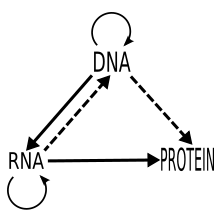
\includegraphics[scale=0.6]{integration/dogma}\centering
    \caption[Central dogma of molecular biology proposed by F. Crick circa 1958]
    {\label{fig:dogma}\textbf{Central dogma of molecular biology proposed by
    F. Crick circa 1958.} The solid lines are proved direct transfer, the dashed
    ones the still have to be proven. Nowadays, we know that the arrow from RNA
    to DNA should be a solid one, even though this happens in very specific
    occasions}
\end{figure}

However, as we still have to prove that proteins can be produced directly
from \DNA\footnote{which seems pretty unlikely to me}, it is assumed that
each protein is created by translation, hence studying
transcriptomics and proteomics together for the same conditions should give us
insights on these regulation processes.

Whereas it was implicitly assumed for a long time that for similar conditions
there should be a proportional relationship between transcriptomics and
proteomics, many studies\
\fixme{add references, see TAC report 3}
done in cells have failed to show high correlation between the two biological
layers. From then, while there are still studies done jointly on transcriptomics
and proteomics, the focus has greatly shift either on the presence or absence of
a protein/transcript in a specific condition or if both transcript and protein
are differential expressed between two conditions in the same way.
Nowadays, there are not many efforts to directly link their actual expression.

Previous studies did not managed to show correlation between proteomics and
transcriptomics above $0.5$ (Pearson correlation coefficient).
However, while cell populations could have external factors impacting their
overall expression, an easy assumption is that tissue samples should be driven
by their function first. As such we expect that what makes a liver a liver and
what makes a heart a heart would overcome most of the technical variability.

In fact, here, even though I have only access to independent data, the average
Pearson correlation per tissue is above $0.5$
[min: $0.45$ (\tissue{Oesophagus}); max: $0.666$ (\tissue{Liver})].

In 2014, two large proteomics assays focusing on normal human tissues have been
released for the first time.
\fixme{add citation for Pandey and Kuster}
Until now, there was not such availability of large-scale and extensive tissues
both on transcriptomic and proteomic layer to jointly study the genes
translation into proteins across a consequent set of tissues
at the same time. Alike the \dataset{Uhlén \etal} dataset and the \dataset{Gtex}
these datasets have not the same scope of tissues. However, the overlap of
studied tissues is enough to draw an overview of the current technology.

In their review,~\citet{Uhlen:2016}, the authors outline one on-going debate
in the literature, which could be formulated whereas we should observe (or not)
good correlations between proteomic and transcriptomic data.
Indeed, first investigations found low or no correlation. More recent
studies reported improved correlations although these correlations were around
$0.4$ (Pearson correlation coefficient). Such discrepancies could be explained
partially by the difference of the technology for proteomic and transcriptomic
assays. Sequencing-based technologies, as \Rnaseq\, enhanced greatly the
assessment of transcripts. While true absolute quantification is not reached yet,
there is not saturation any more or, more importantly, out-of-scope issues as
they could have been observed with microarrays. In theory, on one hand, with
enough sequencing depth, every transcript expressed in a cell or tissue could be
catch by high-throughput sequencing and in the other hand, two transcripts with
different level of expression would be differentiate whereas they are very highly
expressed or not. If there is a difference in their level of expression, this
difference should be catch.

Unfortunately, technology on the proteomic side is not as advanced yet.
Mass spectrometry is still one of the most accurate ways to quantify the
abundance of proteins. However, often the top 25 most abundant proteins can
amount for more than half of the signal collected for a sample. Therefore, the
identification (and hence quantification) of the scarcer proteins is harder.
\fixme{find reference -> ask Jyoti}

These technical divergences and specificities call for an underlying premise:
when is a specific protein or transcript considered as expressed in a dataset?
In a particular tissue?

\begin{comment}
\section{Expressed or not expressed}
\label{sec:IntegrationExpressedOrNot}
While it can seem as a trivial concept and might be overlook, whether a specific
molecule is expressed --- or not --- in a given condition, can actually have
an extensive impact on the results of the analyses, particularly when integrating
proteome and transcriptome together.

Indeed, the Pearson correlation is very sensitive to outliers and null values,
\fixme{Add reference}
hence it is important that the data used for the analysis is meaningful in
its whole.

\begin{figure}[!htbp]
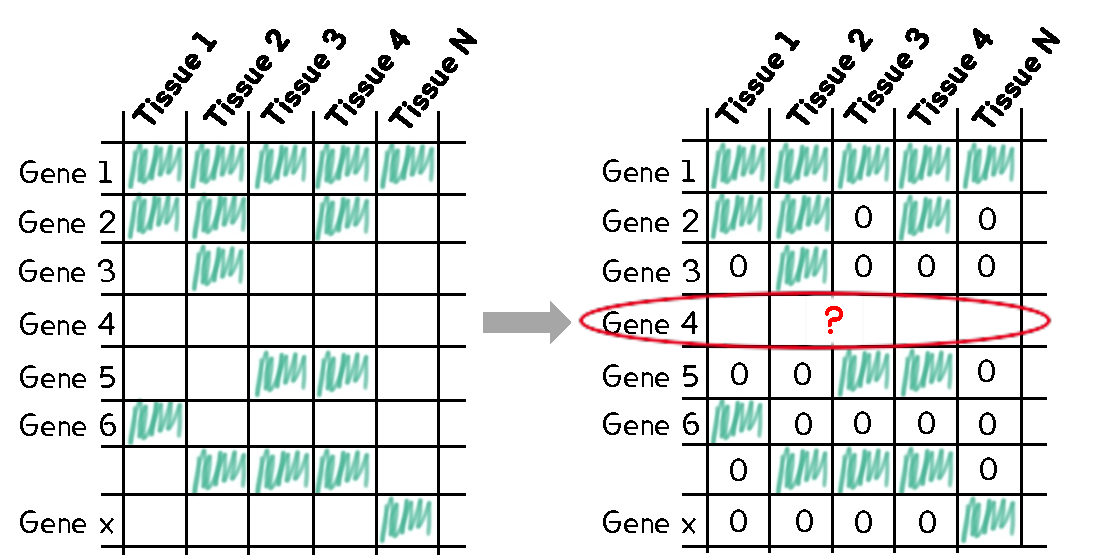
\includegraphics[scale=0.8]{integration/expressedNotExp.pdf}\centering
    \caption[Expressed or not: several cases illustrated]
    {\label{fig:DefineExpression}\textbf{Expressed or not: several cases
    illustrated.}\smallbreak{}Genes as \emph{gene 1} are unequivocal: they have been
    detected in all the different tissues. Genes that have been quantified in
    \emph{some} of the conditions are, in principal, detectable with the
    protocol of sampling and quantification used for the assay.
    For these genes, when no signal is collected, I assume this is a true $0$.
    The genes without any quantification
    in any tissue, e.g.\ gene 4, are discarded from the remaining analysis as
    I can't state
    either there are truly absent from the biological sample or it has to due
    to the protocol at use; they are \emph{undefined}. The same approach is used
    for the transcriptome and the proteome.}
\end{figure}

\subsection{The undefined}\KOMAoptions{parskip=false}
\label{subsec:IntegrationExpressedOrNot-undefined}
If a protein or transcript is never found in any of the samples of a dataset,
then I considered that we can not determine if the protein or transcript was
either truly not expressed or, for any reason, was not capture while the library
preparation or the identification/quantification steps. Hence, those are
excluded from the analyses as I can not resolve precisely if this is a
technical artefact or a biological truth. This case is illustrate by the row
circled in red in~\cref{fig:DefineExpression}.

\subsection{Expression in a dataset}
\label{subsec:IntegrationExpressedOrNot--expDataset}
By contrast, if a protein or a transcript is expressed in some samples of the
dataset, then, whenever no expression was recorded in the other
samples, I consider that the expression of the considered macromolecule is truly
null for those samples.

\subsection{Expression within a sample}
Due to the technical (and biological) differences between proteomics and
transcriptomics, I use different thresholds to define the expression of a protein
or a transcript.

\subsubsection{Expressed protein}
On the proteomic side, I consider that a protein is expressed if it has been
identified and quantified. In other words, if the expression value of a protein
is greater than zero in a sample, I consider it as expressed.

\subsubsection{Expressed transcript}\KOMAoptions{parskip=half*}\label{subsubsec:exprTrans}
It is a bit more complex on the transcriptomic side as there can be
\fixme{find reference on translational noise in RNAseq}
translational noise. While this noise could be evaluate by empirical methods for
each \Rnaseq\ dataset, there is a widespread threshold used in the literature:
$1$ \gls{FPKM} (or \gls{RPKM}). In fact,~\citet{Hebenstreit:2011} showed in
their study \paper{RNA sequencing reveals two major classes of gene expression
levels in metazoan cells}, that to be translated into a protein, a \mRNA\ should
present an expression at least equals to $1$ \gls{RPKM}.

As our current study focuses on the comparison of proteomic and transcriptomic
data, all the analyses have been run with this threshold. It is worth mentioning
that parts of the analyses have also been done either without
any threshold (i.e.\ the same definition used with the proteins has been applied)
or with a threshold of $5$ \glspl{FPKM}.
\end{comment}

\subsection{Limitations of the current study}
Apart of the most obvious limitation: the transcriptome and the proteome used in
this study have been collected from independent human donors, there are
two other main constraints I would like to highlight.

First, there is a lack of samples per tissue on the proteomic side of the study.

On one hand, we have the \dataset{Uhlén \etal} data, which have \emph{technical}
and \emph{biological} replicates for each tissue, and the \dataset{Gtex}, which
provides many \emph{biological} replicates per tissue. On the other hand, no
replicate was produced in the proteomic dataset (\dataset{Pandey \etal}) used
within this study. Hence, the expression found in \emph{one} library is
\textit{de facto} the proteomic expression for that tissue. This
is far from an ideal set-up.

Secondly, while I have compared the list of \emph{undefined} transcripts and
proteins (between \dataset{Pandey \etal} and \dataset{Uhlén \etal} data and
between \dataset{Pandey \etal} and \dataset{Gtex}), I have done the bulk of the
analyses on pairwise (or three-way) \emph{defined} protein and \mRNA(s).

In other words, if the proteins and their corresponding transcripts are not
expressed at least in one sample in each dataset, they are unfortunately excluded
from many many steps of the analysis workflow.

\section{Possible integration approaches}
\label{sec:IntegrationPossibleApproaches}

\begin{figure}[!htbp]
    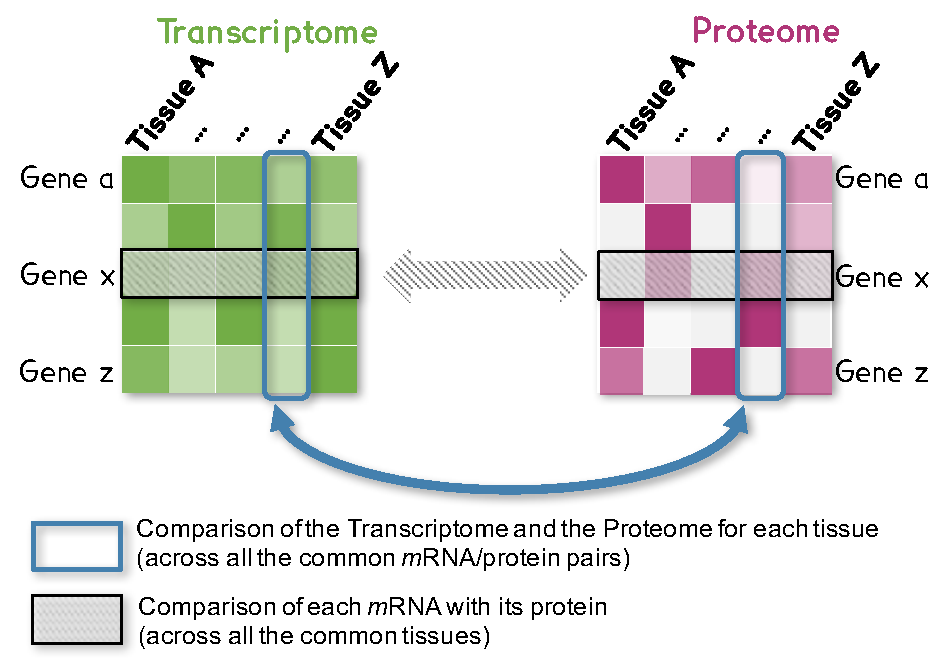
\includegraphics{integration/VisualExplaination}\centering
    \caption[Integration approaches used]{\label{fig:visualexp}\textbf{Integration
    approaches used}
    }
\end{figure}
see \cref{fig:visualexp}

\section{Data}
\label{sec:IntegrationData}

\subsection{Transcriptome}
For this study, the processed \dataset{Uhlén \etal} and \dataset{Gtex} datasets
used are a subset of the processed data previously presented in
the~\Cref{ch:Transcriptomics} (see:~\cref{subsec:Trans_ReproExpresTissue}
for the processing methods). Indeed, only the set of tissues also available
on the proteome side were kept. Parallely, as we are interested to compare each
protein to its corresponding \mRNA\, only the genes annotated as protein coding
for biotype (in Ensembl 76 release) have been kept.

The 14 common tissues between \dataset{Gtex} and the proteomic data
(\dataset{Pandey \etal}) are
(by alphabetical order):  \tissue{Adrenal gland}, \tissue{Bladder}\footnote{Also
sometimes reported as \tissue{Urinary Bladder}},
\tissue{Colon}, \tissue{Frontal cortex}, \tissue{Oesophagus}, \tissue{Heart},
\tissue{Kidney}, \tissue{Liver}, \tissue{Lung}, \tissue{Ovary}, \tissue{Pancreas},
\tissue{Prostate}, \tissue{Spinal cord} and \tissue{Testis}.

The 15 common tissue between \dataset{Uhlén \etal} and the proteomic data
(\dataset{Pandey \etal} are)
an enlarged version of the previous set, with the addition of \tissue{Gall
bladder}, \tissue{Placenta} and \tissue{Rectum}.

Most of the results reported and displayed in the main body
of the following chapter are using this later bigger set. As the whole analysis
pipeline as been applied to the three datasets
for the same 12 tissues, some of the figures have a counterpart in the
appendices displaying the results for all three datasets when focusing only on
that smaller subset of tissues. To ease the comparison, the references of the
supplementary figures are given in green (and in brackets) in the legend of the
main one. Overall, the main results and conclusions remain the same either if
I use Gtex or Uhlén \etal\ data.

To calculate the aggregate expression per tissue\footnote{to be on par with the
proteomic data}, I used the median\footnote{When there were more than
two samples, otherwise it is the mean of expression of the two biological
replicates.} of the transcript expression after having computed the mean of its
expression for the technical replicates of each individual.

I ran the analyses on both quantification (HTSeq and Cufflinks); if not stated
otherwise the quantification used for the figures are based on the normalised
\glspl{FPKM} computed on the output of HTseq.
Overall, either if we use \dataset{Uhlén et al} or
\dataset{Gtex} datasets with any of the quantification methods, the high level
results, discussions and conclusions remain the same.

\subsection{Proteome}
The available data on the proteomic side is by far more limited than the
transcriptomic side. There are really two datasets that could be suitable for
the study: \dataset{Kuster \etal} or \dataset{Pandey \etal} datasets.

While the \dataset{Kuster} dataset presents more tissues in common
with the \dataset{Gtex} and \dataset{Uhlén \etal} datasets
(see~\cref{fig:VennTissuePandeyGtexUhlen}
and~\cref{fig:VennTissueKusterGtexUhlen}), I had focused the study on
the \dataset{Pandey \etal} dataset. Indeed, we managed to quantify the biggest
number of proteins in this later dataset: 10,272 proteins across 24 samples for
\dataset{Pandey} versus 7,223 across 24 samples for \dataset{Kuster}\footnote{Even
if the number of samples is the same for the \dataset{Pandey} and
the \dataset{Kuster} datasets, this is purely fortuitous.}.

\begin{figure}[!htbp]
    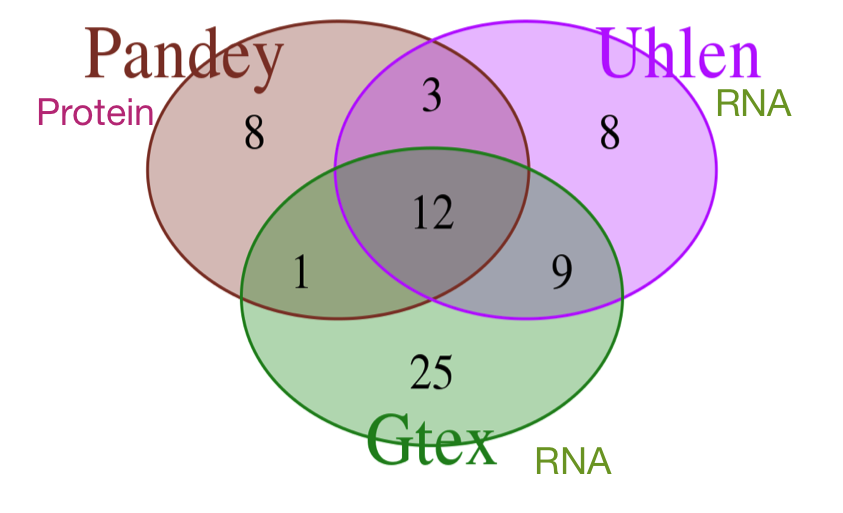
\includegraphics[scale=0.65]{integration/PandeyGtexUhlen_tissuesVenn.png}
    \centering
    \caption[Number of share and unique tissues between the proteomic
    dataset from Pandey \etal\ and the transcriptomic datasets (Uhlén \etal\ and
    Gtex)]{\label{fig:VennTissuePandeyGtexUhlen}\textbf{Number of share and unique
    tissues between the proteomic dataset from Pandey \etal\ and the
    transcriptomic datasets (Uhlén \etal\ and Gtex).} The 12 common tissues of
    the 3 datasets are:
    \tissue{Adrenal gland}, \tissue{Bladder}, \tissue{Colon}, \tissue{Oesophagus},
    \tissue{Heart}, \tissue{Kidney}, \tissue{Liver}, \tissue{Lung}, \tissue{Ovary},
    \tissue{Pancreas}, \tissue{Prostate} and \tissue{Testis}. The 3 added common
    tissue between \dataset{Uhlén \etal} and \dataset{Pandey \etal} are:
    \tissue{Gall bladder}, \tissue{Placenta} and \tissue{Rectum}. The added tissue
    between \dataset{GTEX} and \dataset{Pandey \etal} is the \tissue{Frontal
    cortex}.}
\end{figure}

\begin{figure}[!htbp]
    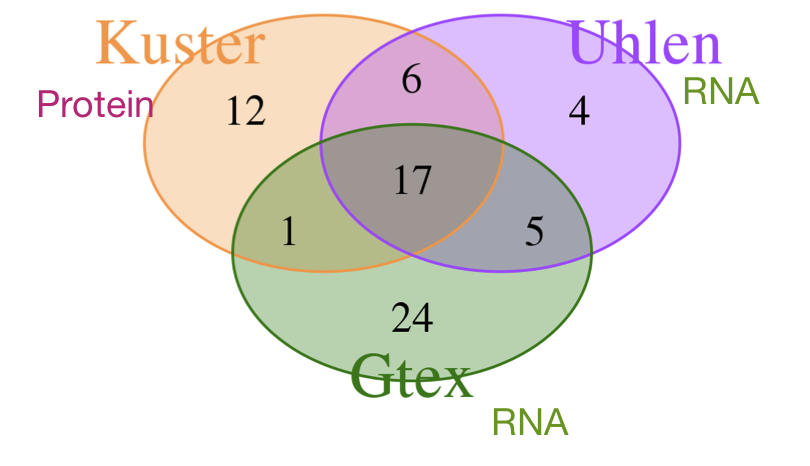
\includegraphics[scale=0.75]{integration/KusterGtexUhlen_tissuesVenn.png}
    \centering
    \caption[Number of share and unique tissues between the proteomic dataset
    from Kuster \etal\ and the transcriptomic datasets (Uhlén \etal\ and
    Gtex)]{\label{fig:VennTissueKusterGtexUhlen}\textbf{Number of share and unique
    tissues between the proteomic dataset from Kuster \etal\ and the
    transcriptomic datasets (Uhlén \etal\ and Gtex).} The 17 common tissues are:
    \tissue{Adrenal gland}, \tissue{Colon}, \tissue{Oesophagus},  \tissue{Heart},
    \tissue{Kidney}, \tissue{Liver}, \tissue{Lung}, \tissue{Ovary},
    \tissue{Pancreas}, \tissue{Prostate}, \tissue{Salivary gland}, \tissue{Skin},
    \tissue{Spleen}, \tissue{Stomach}, \tissue{Testis}, \tissue{Thyroid} and
    \tissue{Uterus}. The 6 added common tissue between \dataset{Uhlén \etal} and
    \dataset{Kuster \etal} are: \tissue{Cerebral cortex}, \tissue{Gall bladder},
    \tissue{Lymph node}, \tissue{Placenta}, \tissue{Rectum} and \tissue{Tonsil}.
    The added tissue between \dataset{GTEX} and \dataset{Kuster \etal} is the
    \tissue{Cervix}.}
\end{figure}

While one could have argue that the greater diversity of proteins in
\dataset{Pandey \etal} data might been due to the nature of the tissues within
each of the proteomic datasets, this is not the case. The number of proteins
detected within a same tissue is greater for  \dataset{Pandey \etal},
as shown in~\cref{fig:KusterPandeyFQM} (A and B).

This has an increased importance as the study goes beyond the correlation of
proteomics and transcriptomics for a same tissue.

\newcommand{\figKustPandFQM}{\textbf{Distribution of proteins across the
tissues.}\\The tissues are ordered by the number of different proteins they
expressed. Highlighted in red are the proteins that are found solely in that
tissue (within each dataset).
A\textbar\ Kuster (first quantification method).
B\textbar\ Pandey (first quantification method).
C\textbar\ Pandey (second quantification method).
There are by far many more detected and quantified proteins per tissue in the
\dataset{Pandey \etal} dataset (B\textbar) than the
\dataset{Kuster \etal} dataset (A\textbar). We can notice that while
\tissue{Testis} is the tissue that presents the highest number and greatest
diversity of expressed proteins for both datasets, the other tissues are not in
the same order.}


%\ifthispageodd{\afterpage{\clearpage\
\begin{figure}[!htbp]
% 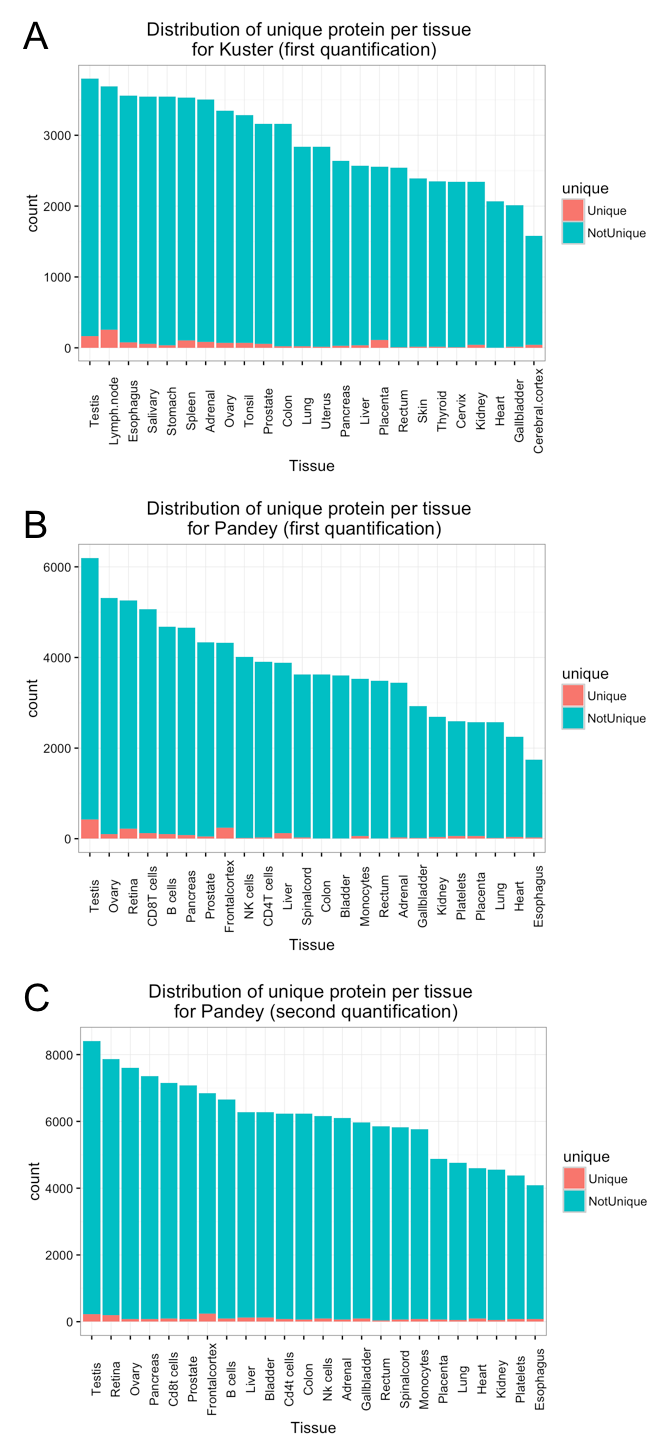
\includegraphics[scale=0.90]{integration/KusterPandey1_2FQM.png}\centering\label{fig:KusterPandeyFQM}
%\end{figure}
%\captionof{figure}[Distribution of proteins across the tissues]{\figKustPandFQM}
%}}{\begin{figure}
% 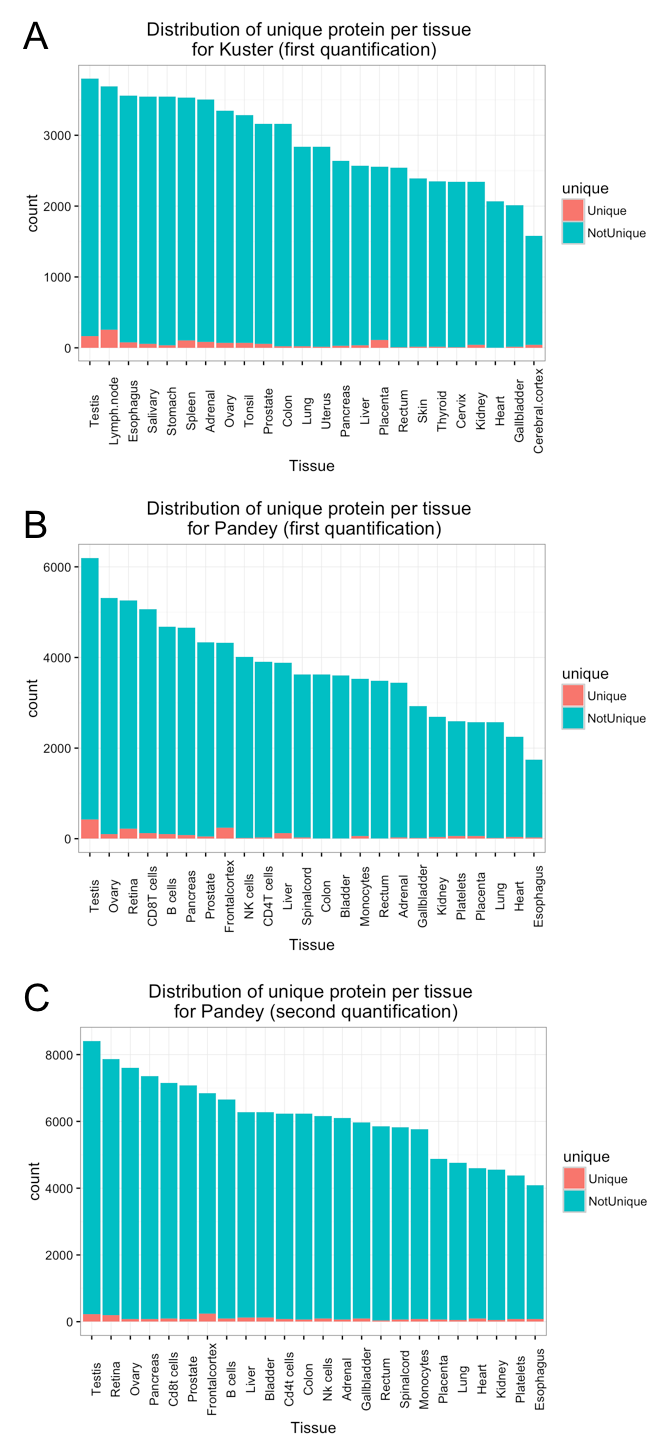
\includegraphics[scale=0.90]{integration/KusterPandey1_2FQM.png}\centering\label{fig:KusterPandeyFQM}
    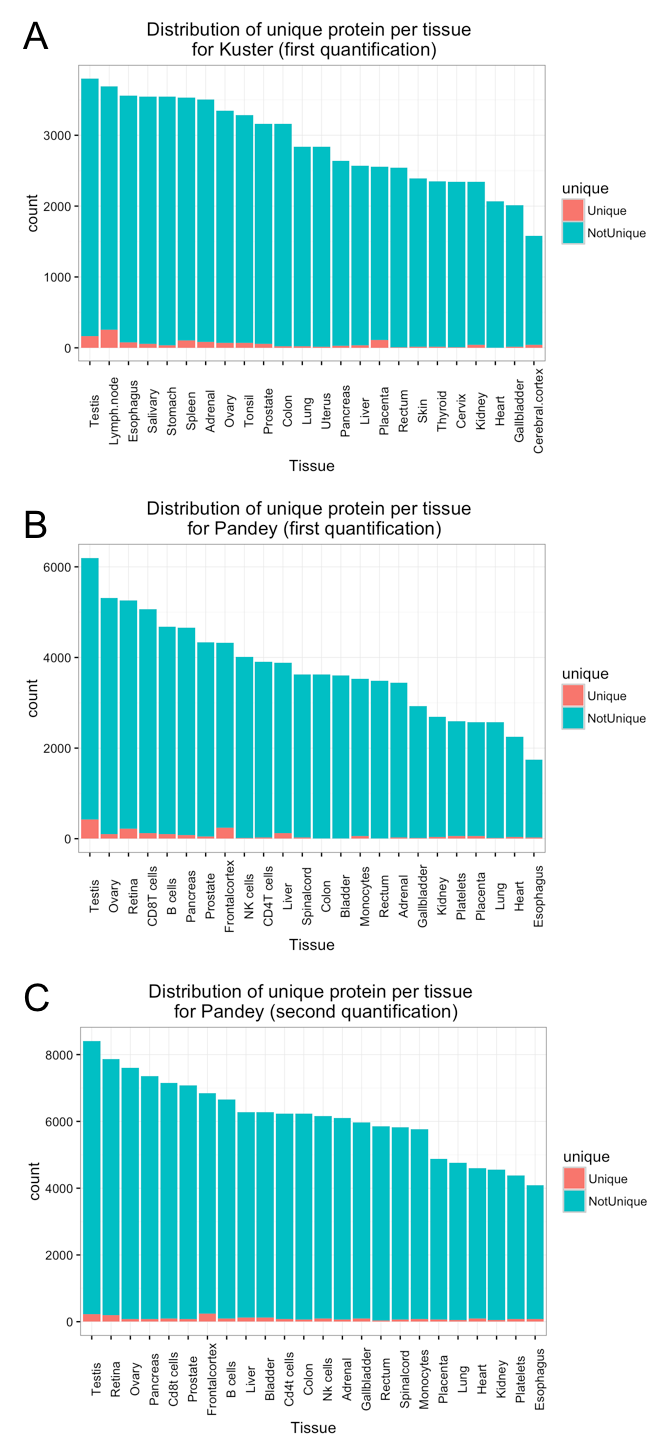
\includegraphics[scale=0.75]{integration/KusterPandey1_2FQM.png}\centering
    \caption[Distribution of proteins across the
    tissues]{\label{fig:KusterPandeyFQM}\figKustPandFQM}
\end{figure}
%\captionof{figure}[Distribution of proteins across the tissues]{\figKustPandFQM}
%    }

Furthermore, all the \dataset{Pandey \etal} data has been
collected on the same platform while the \dataset{Kuster \etal} data has been
collected on different ones. On a side note, as each of the proteomic datasets
proposes only one sample per tissue, it is difficult to assess if the high or low
correlation between the \dataset{Kuster \etal} or the \dataset{Pandey \etal}
proteomic data and the available transcriptomic data is due to the technology or
to the nature of the tissue.

In the same fashion as the transcriptomic data, which have been reprocessed
before being employed in our studies, the proteomic data have been reprocessed
by James from the raw files he has downloaded from ProteomeXchange
\citep{ProteomeXchange:2014} via the PRIDE database \citep{Pride:2016}.
\fixme{Ask James for the methods}

At first, the quantification used for the proteomic data was following
state-of-the-art protocols for which we applied very stringent parameters:
to identify and quantify a given protein, three different unique peptides
(with a \gls{FDR} $< 0.01 \%$) have to be mapped solely to that protein. A main
issue of this approach is that many proteins have similar sequences; hence, some
peptides can only be attributed to clusters of proteins. A naive approach would
be to aggregate the corresponding transcriptomic expressions together to enable
the comparison\footnote{Which then would also require further steps of
normalisation on the transcriptomic part.}. However, we found that the cluster
of peptides/proteins are not consistent from one study to another. Indeed, we do
not always observe the same set of peptides and, moreover, the proteins clusters
they support are quite different. That is why I have not investigate this option
further as for each study I would need a new aggregate annotation as a reference.
It would then be quite difficult to assess the discrepancy due to the
variations of aggregation. For this first method of quantification, I choose to
exclude the cluster of peptides/proteins from the study\footnote{Since I also work
with a subset of the tissues, out of context, the number of quantified proteins
could seem a bit low compare to the original study.}.


\section{Results}
\label{sec:IntegrationResults}

\subsection{New quantification method for the proteomic data}
\label{subsec:IntegrationNewMethQuant}

\textit{Quantifications performed by Dr James Wright}

After discussions where we were comparing the different quantification algorithms
and methods used for \Rnaseq\ data, we have decided to try a new quantification
method\footnote{Inspired by algorithms as Cufflinks} for the proteomics:
the amount of proteins would still take in account the \emph{unique} peptides,
but also the peptides that could be attributed to several proteins.
These \emph{ambiguous} peptides are then probabilistically assigned to the
mapped proteins they are more likely to come from (based on the distribution of
the other peptides that could be mapped to each protein).

Both quantification methods have been implemented by James Wright.

In the context of this work (i.e.\ when focusing on the 15 common tissues between
the \dataset{Uhlén \etal} and the \dataset{Pandey \etal} datasets),
he has quantified about 6,400 proteins with
the standard method. With the new method, he has quantified a bigger set of
proteins: about 12,300 proteins. This new number is quite closer to the original
reported number of protein by Kim \etal\.  Indeed the original paper is
reporting proteins encoded by 17,294 genes.

As shown in~\cref{fig:KusterPandeyFQM} (B and C),
all tissues and cell lines benefits from this new quantification and there isn't
any tissue or cell line that is dramatically impacted compared to the others.

As shown in~\cref{fig:VennGeneTransProt15}, there are 14,617 pairs of
proteins/genes. While, we expect a greater number of transcripts than proteins,
it could however be primarily surprising that there are proteins
(See supplementary Table~\cref{tab:protNoTrans}) which don't have
a match in the transcriptomic data. There are actual several possible explanations.

\begin{figure}[!htbp]
    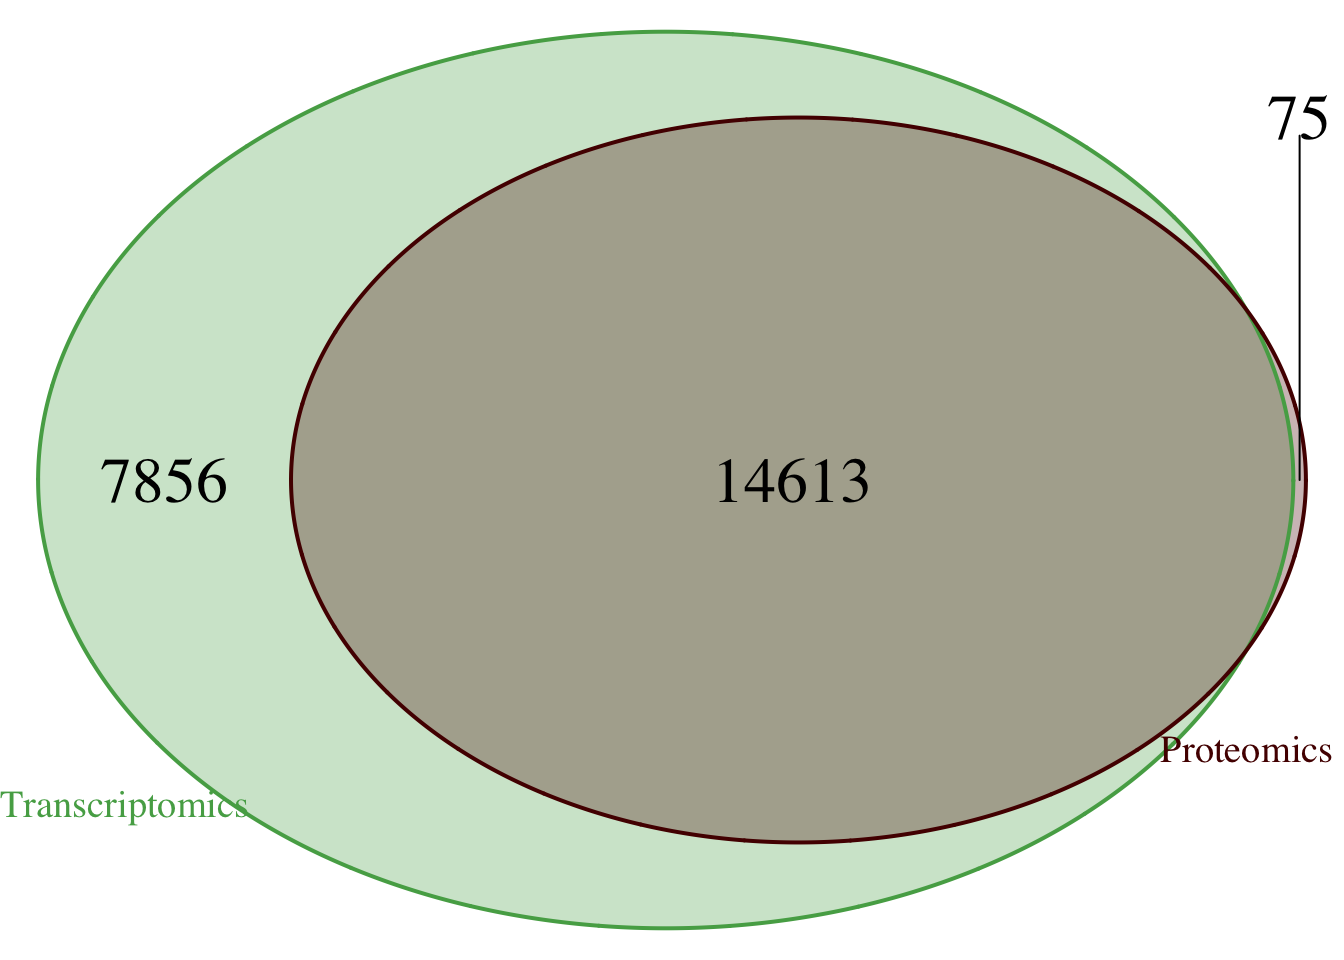
\includegraphics[scale=0.15]{integration/VennGeneTransProt15}\centering
    \caption[Unique and shared protein/gene pairs between Proteomics
    (Pandey \etal\ (PPKM)) and
    Transcriptomics (Uhlén \etal\ (\gls{FPKM}))]
    {\label{fig:VennGeneTransProt15}\textbf{Unique and shared protein/gene
    pairs between Proteomics (Pandey \etal\ (PPKM)) and Transcriptomics (Uhlén
    \etal\  (\gls{FPKM})).} There are 14,613 pairs common between the
    transcriptomic (only the protein coding genes are considered)
    and the proteomic dataset.}
\end{figure}

It could be a technical issue or an artefact on the transcriptomic side, e.g.\
the \mRNAs\ were present but were not capture for a reason or another at the
library preparation step; the \mRNAs\ have a high sequence-similarity with other
\mRNAs\ and the reads haven't been accurately assigned; the lacking \mRNAs\ are
not properly annotated in the version of the genome I used at the mapping step.

It might also be that the protein doesn't belong to the sample: the identification
is a false positive or incorrect; the sample\footnote{Or the instrument used for
the capture} might also have been contaminated at some point with some foreign
proteins.

It can also be due to an underlying biological phenomenon:
the turnover of the \mRNA\ is very low, while the protein is very stable;
the proteins have been expressed somewhere else and then has been imported in the
current tissue (e.g.\ hormones or cytokines). Finally, as the proteome
and transcriptome used for this study have been collected independently, if the
gene is individual- or population-specific, we will then detected in one of the
study and not in the other one. However, as we have biological replicates on the
transcriptomic side, this last hypothesis seems the most unlikely.
Of course, a mixture of the previous causes is also highly probable.

I have performed the analyses presented in this chapter on both sets of
quantification. As the high-level results and conclusions are remaining the same,
the figures and discussions hereafter are based on
the new quantification method. For comparison purposes,
I have produced (following the same analyses and with their associated
implementations) some figures and tables from the data quantified by the first
method. Those can be found in the appendices; their references
are given in blue (and in brackets) in the caption of the main figures.

In the following sections, we consider the proteomic data with this new
quantification method and compare it to the \dataset{Uhlén \etal} dataset
for their 15 common tissues.

\subsection{Expression profile of proteomics and transcriptomics look very
similar in shape on a logarithmic scale}
\label{subsec:IntegrationExpProfileSim}

As discussed in the previous chapters, visualising the data is very important
prior to any computation. It allows to detect if we are violating
any assumption or if there is any issue with the data. In fact, we have seen
in~\cref{ch:Transcriptomics} that there is an issue with the pancreatic
samples for the \dataset{Uhlén \etal}, as the range of genes expression is quite
different from the other samples/tissues.

Considering the scale of expression between the proteomic assay and the
transcriptomic ones, they are not directly comparable. Hence,
all the data (regardless of the method of quantification) have been transformed
with $X_{i}=\log_{2} (x_{i}+1)$ (or $X_{i}=\log_{2} (x_{i})$)
before any other computation or visualisation.


\begin{figure}[!htbp]
    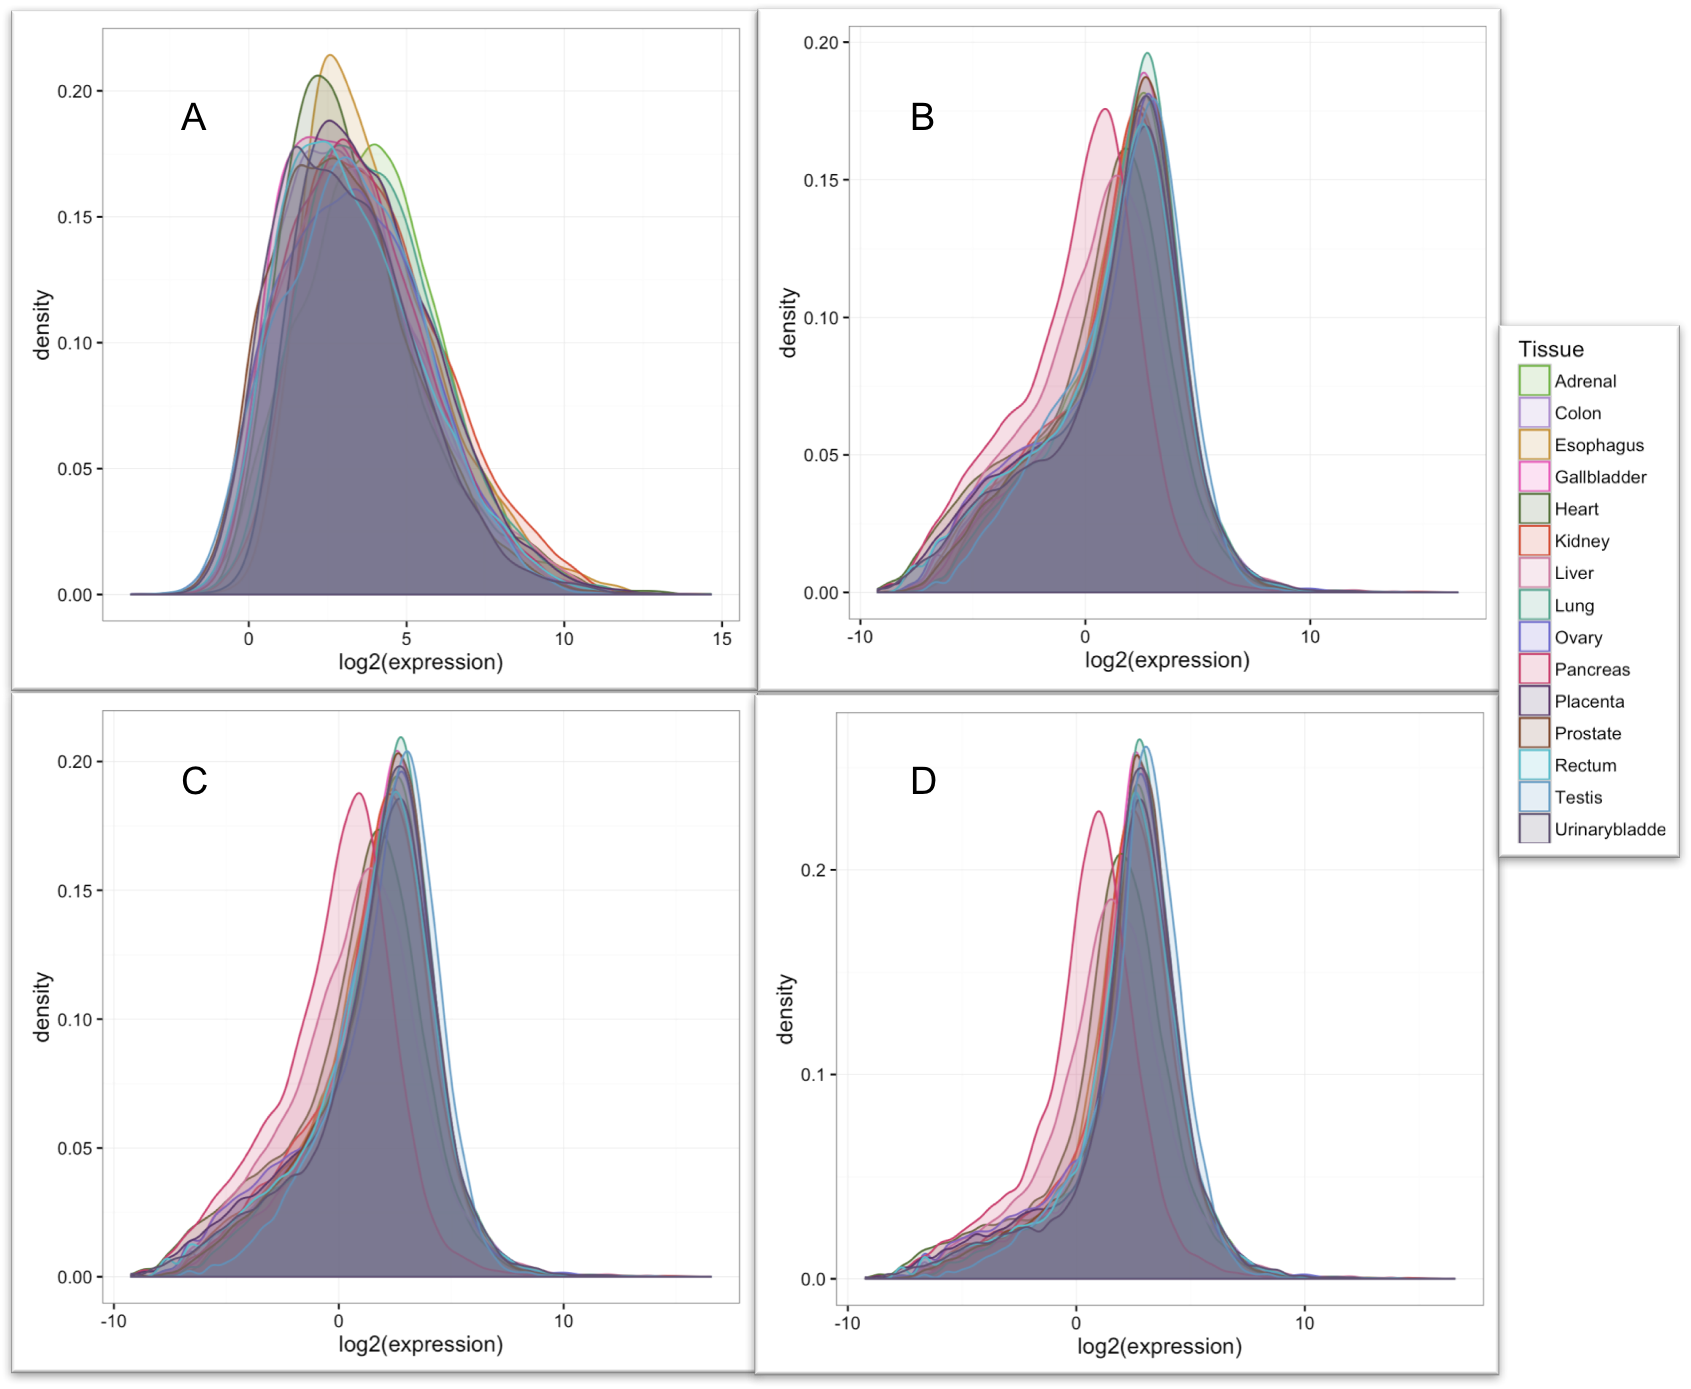
\includegraphics[scale=0.45]{integration/densityExpProtTrans15}\centering
    \caption[Density of expression of proteins and \mRNAs\ per
    tissues.]
    {\label{fig:densityExpProtTrans15}\textbf{Density of expression of
    proteins and \mRNAs\ per tissues.} \\\textbf{A}| Proteins.
    \textbf{B},\textbf{C},\textbf{D} present the same data but with
    different thresholds:
    \textbf{B}| No threshold. \textbf{C}| 1 \gls{FPKM}.
    \textbf{D}| 5 \glspl{FPKM}.\\The threshold used for the proteins is the
    threshold of
    detection (i.e.\ greater than zero). The different density of distributions are
    globally gaussian. When the threshold is increased for the transcriptome, the
    shape get closer to the ideal one, as the bulge created by lowly expressed
    genes is removed. We can also observe that the problem with the pancreatic
    tissue get more highlighted with higher thresholds.}
\end{figure}

\Cref{fig:densityExpProtTrans15} presents the density of expression
of proteins and \mRNAs\ per tissue. In~\cref{fig:densityExpProtTrans15}|A,
we notice that the densities of expression of the proteins have a similar gaussian
shape for each of the tissues. We can also observe than the expression values
of the proteins gather towards the very low values.
In~\cref{fig:densityExpProtTrans15}|B to~\cref{fig:densityExpProtTrans15}|D,
we can observe the density of expression values for
the \mRNAs\ across all the tissues for
different threshold cut-off: $0$, $1$ and $5$ \glspl{FPKM}.
We remark that when we increase the threshold, the shape
of the density becomes closer to a lorentzian.~\Cref{fig:densityExpProtTrans15}|B
displays the density of expression for \emph{any} detected \mRNA\@. We can
then observe a bulge composed by the very lowly expressed \mRNAs\, for which it
is hard to decipher which are the one that are translated into proteins and which
should be considered as translational noise. When I use $1$ \gls{FPKM} as a threshold,
we observe density curves that are closer to the ideal one and these \mRNAs\ are
more likely translated into proteins.

\TK{NEED TRANSITION to comparison tissue levels for the two layers!}

\subsection{Independently human sourced transcriptomics and proteomics
have good and significant correlation for same-tissue pairs.}
\label{subsec:IntegrationGoodCorrProtTrans}

I used the whole set of common expressed \mRNAs\ and
expressed proteins\footnote{Without any other constraint: e.g.\ the \mRNA\ and
its corresponding protein do not have to be detected in the same tissue.}.
Then, I calculated the correlation between the proteome and the trancriptome for
each tissue, i.e.\ for each tissue, I compared each protein expression value to
its corresponding gene one.

As I exposed in~\Cref{ch:Transcriptomics}, there are some
\mRNAs\ that are lowly or even anti-correlated between the different
transcriptomic datasets.
As I can not pinpoint whether this is due to \emph{biological} or \emph{technical}
reasons, we choose to exclude the anticorrelated \mRNAs\ between \dataset{Uhlén
\etal} and \dataset{Gtex} (across the 23 common tissues) as these two datasets have
very similar protocols and have been sequenced on similar sequencers (Illumina
HiSeq 2000/2500).

As illustrated in the supplementary~\cref{fig:ScatterPlotLiver}
and~\cref{fig:ScatterPlotOesophagus}, while the exclusions of these genes might
slightly improve some of the results, it can also have a feeble opposite effect
in some other cases.
Indeed, some pairs of \mRNA/protein might have a very tight relationship in some
tissues and looser in others. Whilst this could be due to technical reasons, it
could also be due to biological ones. Unfortunately, with our current knowledge
of the datasets, it is not possible to reject pairs \emph{a priori}.

In this context, the range of Pearson correlation coefficients between the
proteomic and the transcriptomic data is from $0.66$ for the \tissue{Liver}
to $0.46$ for the \tissue{Oesophagus}.\footnote{\textbf{NB}: If I exclude the
pairs where the \mRNA\ is expressed below $1$ \gls{FPKM}, the Pearson correlation
coefficients for each tissue are substantially identical.}

\begin{figure}[!htbp]
    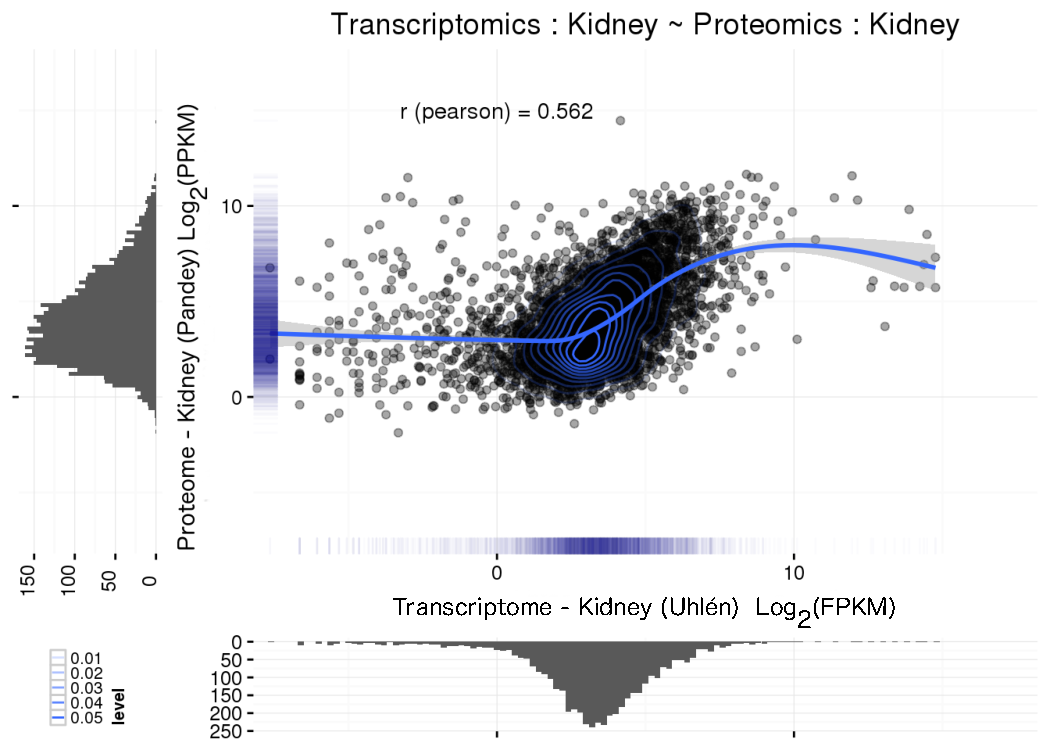
\includegraphics[scale=0.85]{integration/Kidney_scattplot.pdf}\centering
    \caption[Scatter plot of the expression value of the proteins (Pandey)
    and the \mRNAs\ (Uhlén \etal) for Kidney]
    {\label{fig:ScatKid}\textbf{Scatter plot of the expression value of the
    proteins (Pandey) and the \mRNAs\ (Uhlén \etal) for Kidney.}
    This scatter plot displays the
    log-transformed ($Log_{2}$) expression value of
    each \mRNA\ on the x-axis and the log-transformed ($Log_{2}$)
    expression value of the proteins on the
    y-axis. Each point represents a corresponding pair of \mRNA\ and protein.
    We can notice that most of the \mRNA/protein pairs are very close to
    the diagonal, which indicates a high correlation between the level
    of \mRNAs\ and proteins. We also see that the lower levels of expression of
    \mRNAs\ are more prone to the dispersion ($<0$ on $Log_{2}$-scale, so $<1$
    \gls{FPKM} on the original scale, which is a common threshold used for the
    coding \mRNAs). Besides, the proteins present most-likely a
    saturation effect of their expression values. The highest expressed protein
    is \protein{\gls{HBB}}
    (i.e.\ Hemoglobin Subunit Beta) which is also found in the 5 highest
    expressed proteins in all the other tissues. It is quite likely that for
    most of the tissues, this is due to how they have been sampled.
    \\The distributions of the proteins and the \mRNAs, plotted on the outer part
    the figure, have similar shaped.\\
    \textbf{N.B.:} Whilst every pair of \mRNA\ and protein has been used to
    calculate the correlation, the pairs with a null element have been not plotted
    to optimise the visualisation.}
\end{figure}

\Cref{fig:ScatKid} illustrates the comparison of the proteomic data to the
transcriptomic data for the \tissue{Kidney} which stands within the middle of the
correlation range as its coefficient is equal to $0.56$.
The x-axis represents the level of the \mRNAs\
expression on a $Log_{2}$-scale and the y-axis represents the levels for the
proteins (also on a $Log_{2}$-scale). Whilst, every pair of \mRNA\ and
corresponding proteins has been used to calculate the overall Pearson correlation
coefficient, the pairs with a null element have been excluded from the plotting
to optimise the visualisation. As we can see, there is a higher dispersion for
small expression values of \mRNAs\ (lesser than $0$ $Log_{2}$(FPKM), i.e.\
$1$ FPKM). This dispersion could be due to technical limitations or translational
noise (see \cref{subsubsec:exprTrans}). For the highly expressed \mRNAs\ side,
we can observe a possible saturation effect on the proteomic side. These two
phenomenon explain why the correlation coefficient value is so low when the
bulk of the protein/\mRNA\ pairs present a positive strong and quite linear
association.

When I perform the previous comparison for the remaining 14 tissues, the results are
quite similar (see~\cref{fig:ScatterPlotAll}). To test the significance of these
coefficients, I have also calculated the Pearson correlation coefficients of
random pairs of tissues, i.e.\ instead of comparing the $Proteome_{Adrenal}$ with
the $Transcriptome_{Adrenal}$, (which is a \emph{same tissue pair} comparison),
I compare for example the $Proteome_{Adrenal}$ with the $Transcriptome_{Placenta}$.
(see~\cref{fig:TestSig})

\begin{figure}[!htbp]
    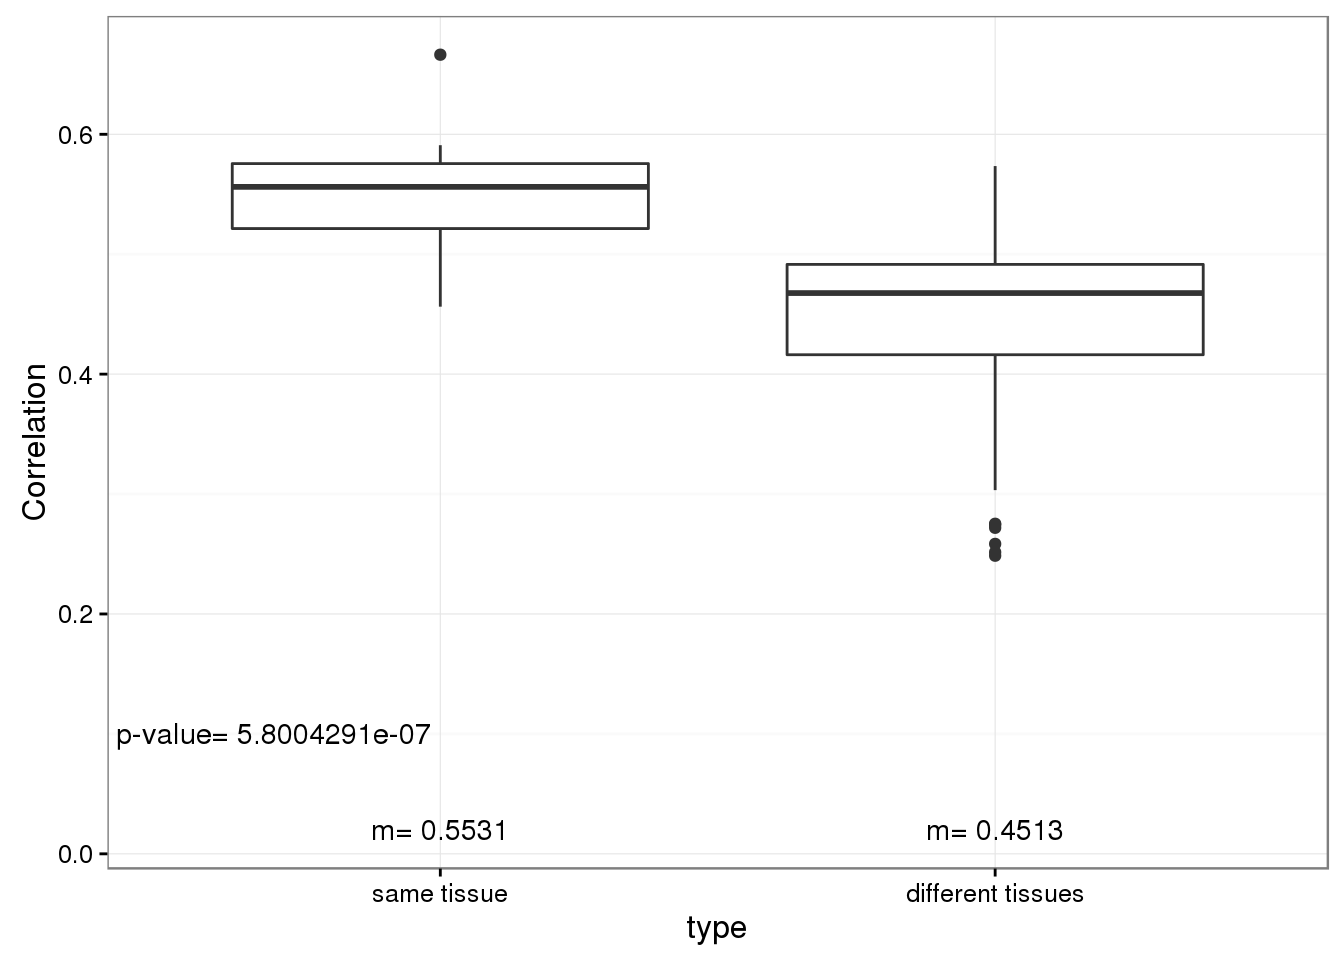
\includegraphics[scale=0.55]{integration/TestWhole_withoutLow.png}\centering
    \caption[Distribution of Pearson correlation coefficients for same tissue
    pairs versus random tissue pairs]{\label{fig:TestSig}\textbf{Distribution of
    Pearson correlation coefficients for same tissue pairs versus random tissue
    pairs.} The left boxplot displays the distribution of Pearson correlation
    coefficients for same tissues pairs (e.g.\
Proteome\textsubscript{\tissue{Liver} }$\sim$Transcriptome\textsubscript{\tissue{Liver} }
or
Proteome\textsubscript{\tissue{Heart} }$\sim$Transcriptome\textsubscript{\tissue{Heart} }).
    \\The right boxplot shows the correlation of all the possible random
    pair of tissues (e.g.\
Proteome\textsubscript{\tissue{Lung} }$\sim$Transcriptome\textsubscript{\tissue{Liver} }
or
Proteome\textsubscript{\tissue{Heart} }$\sim$Transcriptome\textsubscript{\tissue{Kidney} }).
    A Welch t-test has been performed to test the significance of the
    difference of the means of the two groups ($0.55$ for the same tissue and
    $0.46$ for the random pairs). The difference is significant under the null
    hypothesis $H_{0}$ (The mean of the same pair-tissue coefficient correlations
    is higher than the random tissue pairs for a confidence interval of $95\%$:
    p-value: $5.8e-07$).}
\end{figure}

\fixme{citation for Welch t-test}

\TK{transition: we know that the overall expression profiles are closely associated.
Next point is to check if a higher specificity of the proteome of a tissue is due
to a greater specificity at transcriptome level.}

\subsection{Uniqueness of a protein can not be deduced by the uniqueness of a
\mRNA}
If we consider \cref{fig:KusterPandeyFQM},
(particularly \cref{fig:KusterPandeyFQM}|C), we can see that for every tissue,
there are proteins only detected in that specific tissue. This is also the case
for the transcriptome, some \mRNAs\ have been detected in only one tissue.
\Cref{fig:barPlotunique0nb} shows the amount of \mRNAs\ and proteins that have
been \emph{detected} in each tissue. The number of \mRNAs\ is actually quite
high. However, the limit of detection for \mRNAs\ does not imply that these \mRNAs\
are translated into proteins or that they are specific to the tissue. Indeed,
as I have presented previously (see~\Cref{ch:Transcriptomics}),
most of the \mRNAs\ are detected everywhere.

Hence, as a second approach, I only used the \mRNAs\ expressed
above $1$ \gls{FPKM} (see \cref{fig:barPlotunique1nb}). Independently of
thresholds, \tissue{Testis} presents --- consistently --- the highest number
of unique proteins and \mRNAs. We can also observe that the number of \mRNAs\
detected is roughly equivalent to the number of \mRNAs\ quantified only once at
least at (or greater than) $1$ \gls{FPKM} although these \emph{unique} genes are
not exactly the same.

As there is an obvious bias towards the low expressed \mRNAs\
(which are usually part of the least correlated pairs of \mRNA/proteins), I also
used a threshold of 5 \glspl{FPKM}. This last threshold, albeit purely arbitrary,
has already been used in the literature and presents some similarity regarding the
breadth of expression of \mRNAs\ with the proteins' one
(see \cref{subsec:IntegrationProteinBimodalExpre}).

\TK{insert reference here --- check cancer studies}

At this threshold, the number of \emph{unique} \mRNAs\ is lesser than previously,
but still greater than the number of \emph{unique} proteins (see
\cref{fig:barPlotunique5nb}).

Once again, there is not any obvious relation between
what we observe on the proteomic side and the transcriptomic one.
In \cref{fig:barPlotunique5ratio}, I used the ratio of the number of \emph{unique}
\mRNAs\ per tissue divided by the total amount across all the tissues.
Hence, we can easily see that while \tissue{Testis} presents more than half of
the \emph{unique} \mRNAs\, it represents less than a quarter of the diversity
at proteomic level.

\begin{figure}[!htbp]
    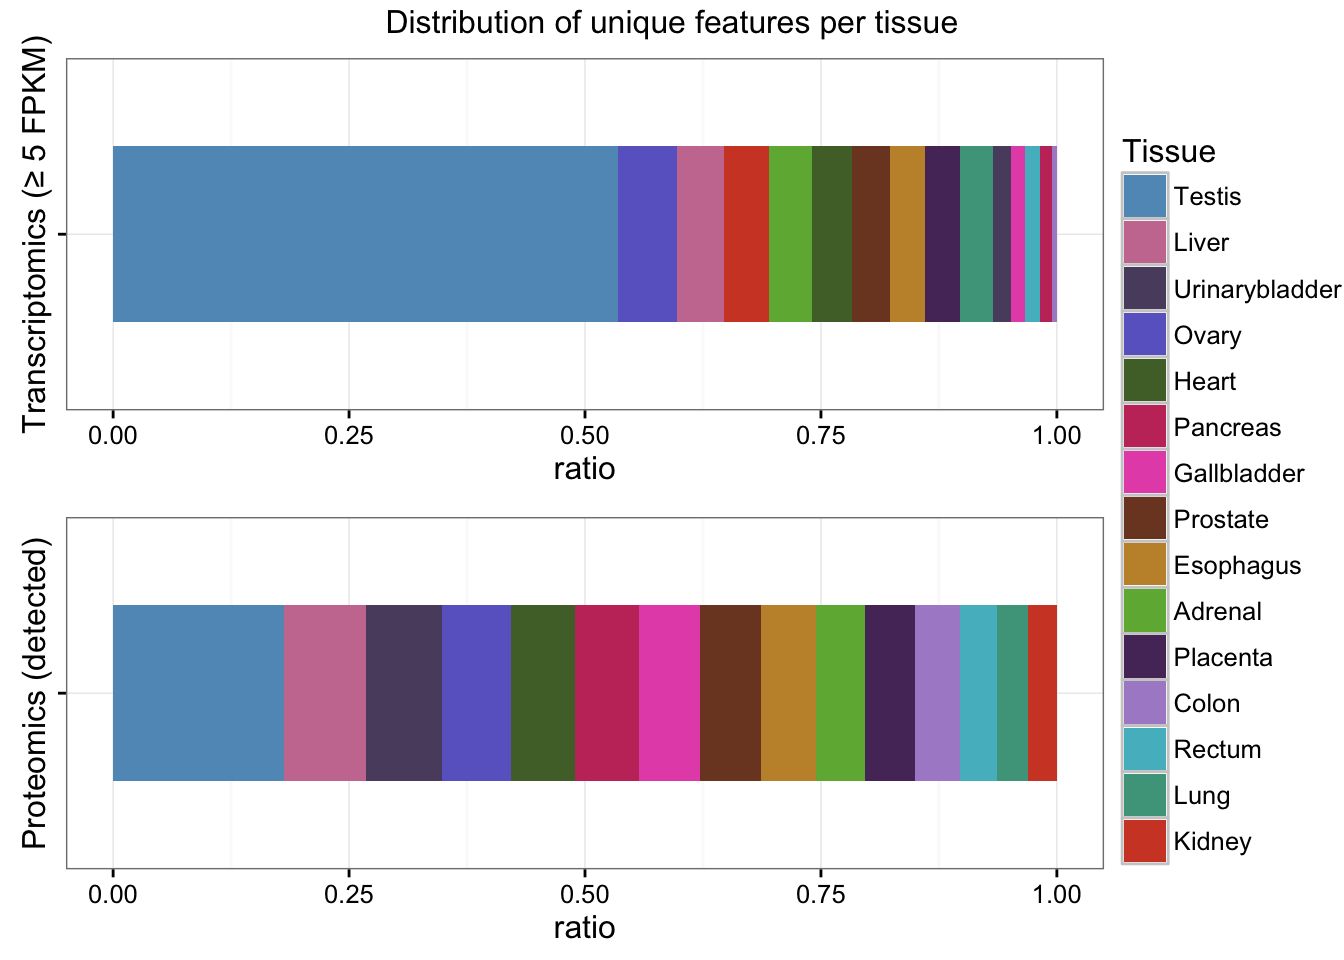
\includegraphics[scale=0.30]{integration/barPlotunique5ratio}\centering
     \caption[Distribution of \mRNAs\ and proteins detected (at specific
     thresholds) only in one unique
     tissue]{\label{fig:barPlotunique5ratio}\textbf{Number of
     \mRNAs\ (top) and proteins (bottom)
     that have been detected and quantified (\geq\ 5 \glspl{FPKM} for \mRNA\;
     \textgreater\ 0 for proteins).} While some tissue can have
     consistently a higher
     specificity at proteomic and transcriptomic level, it is not true for all.}
\end{figure}


\subsection{Distribution of expression breadth of the proteome is bimodal. As is
the expression breadth of the mRNAs --- if we apply a threshold}
\label{subsec:IntegrationProteinBimodalExpre}
\fixme{this probably need to go to the previous chapters!}

In our study, most proteins are detected in a very limited number of tissues (one
or two) or in all the tissues as it can be observed in~\cref{fig:breadthProt}.
Overall, we found that most proteins are found in one tissue. We refer to them as
\emph{tissue-specific}.

\begin{figure}[!htbp]
    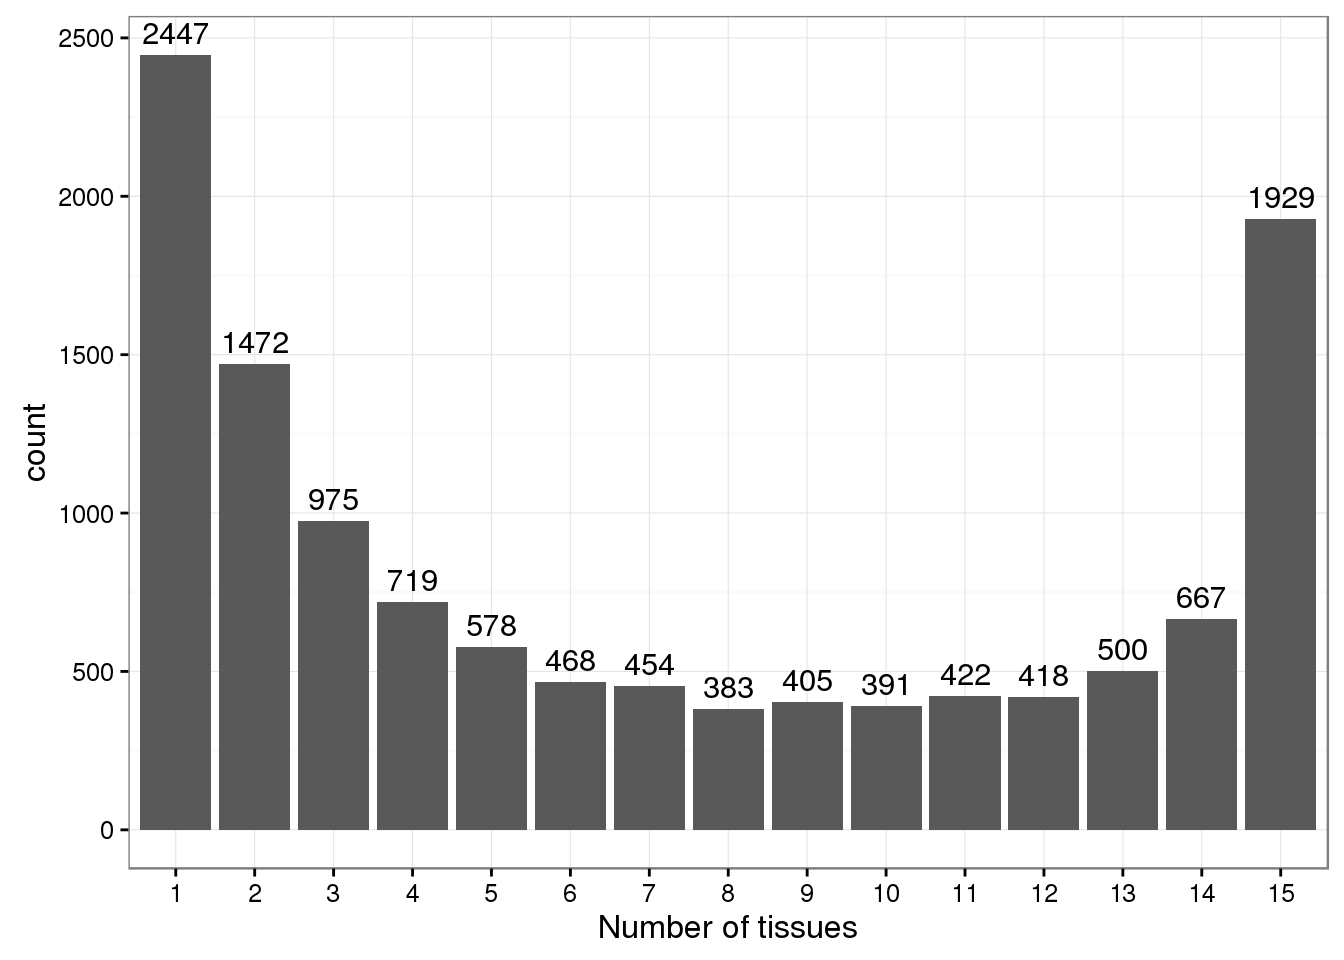
\includegraphics[scale=0.65]{integration/breadthProt.png}\centering
    \caption[Distribution of expression breadth for the proteome]
    {\label{fig:breadthProt}\textbf{Distribution of expression breadth for the
    proteome.} The breadth of expression is bimodal: most of the proteins are
    only found in one tissue. The second largest group is consisting of
    the ubiquitous proteins. The third largest group is the group of the proteins
    that are expressed in two tissues.}
\end{figure}


For the transcriptome, if we focus only on the detected genes, we don’t observe
the same trend as showed in~\cref{fig:breadthTrans}|A.
However, when we apply a threshold, either $1$ \gls{FPKM}
(\cref{fig:breadthTrans}|C) or
5 \glspl{FPKM} (\cref{fig:breadthTrans}|D), to which the \mRNA\ expressions
have to be greater or at least equal, then the expression breadth distribution
of the \mRNAs\ is also bimodal.

\begin{figure}[!htbp]
    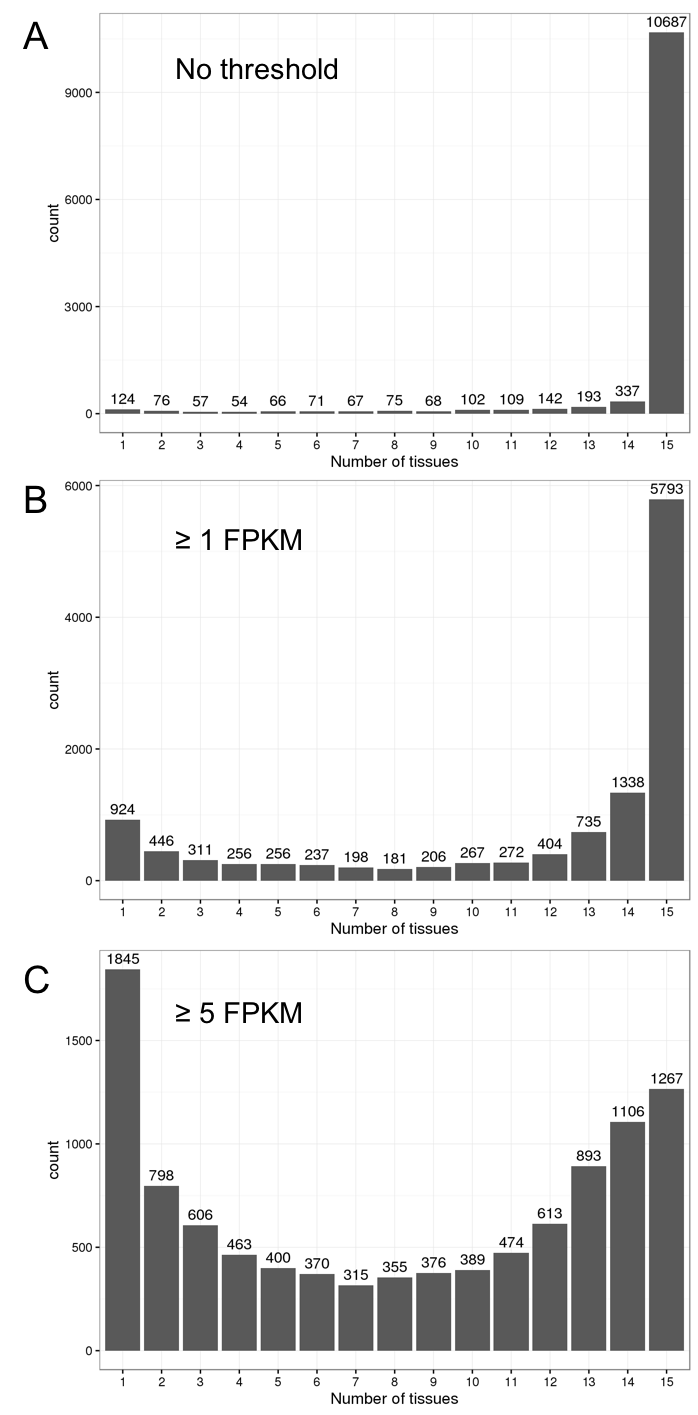
\includegraphics[scale=0.85]{integration/breadthTrans}\centering
    \caption[Distribution of expression breadth for the transcriptome]
    {\label{fig:breadthTrans}\textbf{Distribution of expression breadth for the
    transcriptome.} The distribution is given for several threshold.
    \textbf{A}| Every time a \mRNA\ is detected ($> 0$ \gls{FPKM}).
    \textbf{B}| Every time a \mRNA\ is detected at or above $1$ \gls{FPKM} and
    \textbf{C}| $5$ \glspl{FPKM}.}
\end{figure}

\subsection{Few protein expression breadth can be predict by transcript
expression breadth}

\begin{figure}[!htbp]
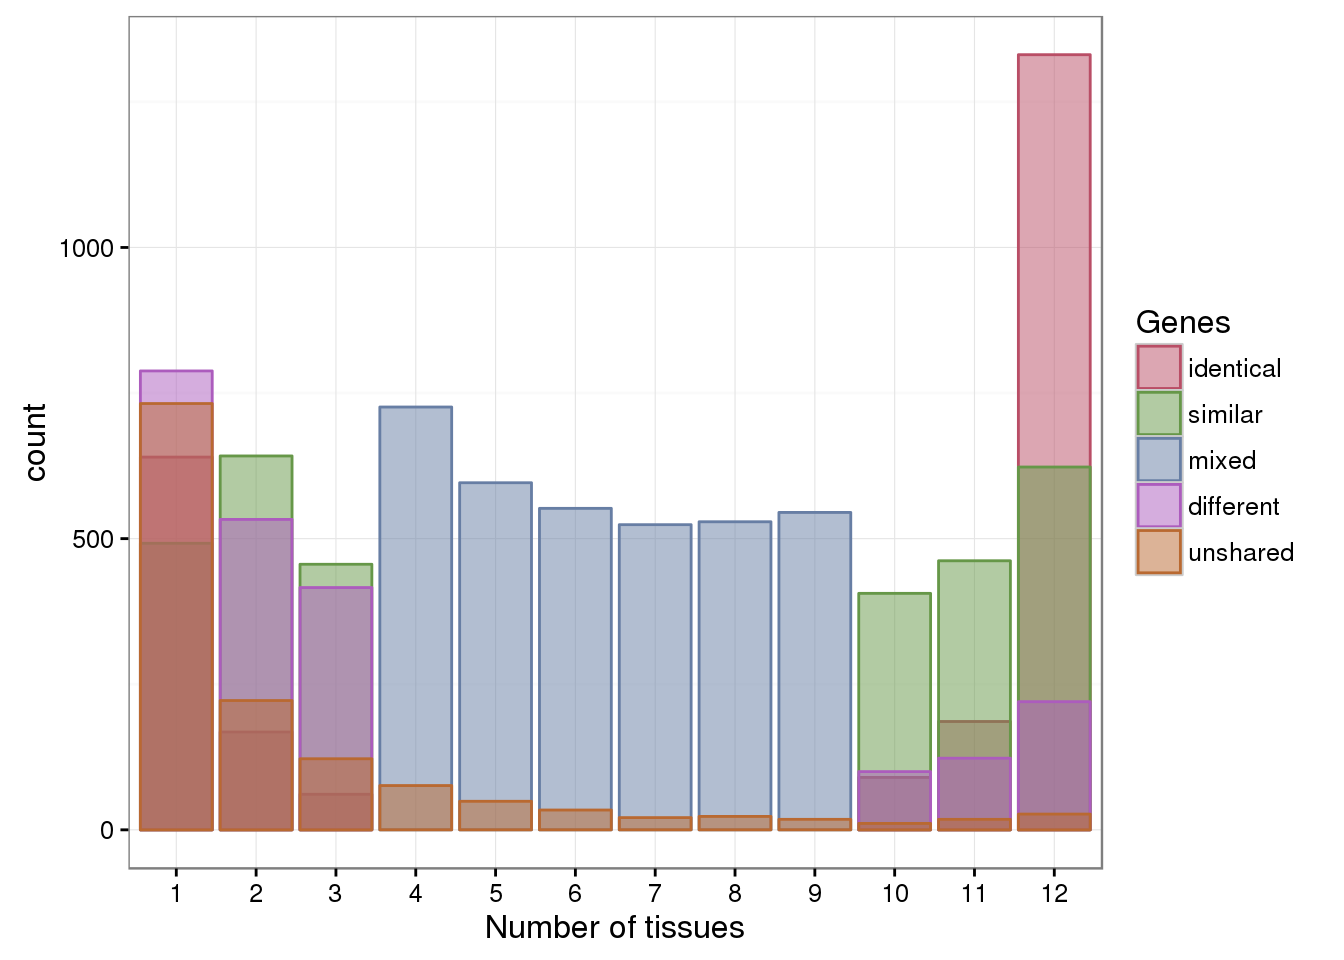
\includegraphics[scale=0.30]{integration/PandeyUhlenAnnoBreadth}\centering
    \caption[Proteome expression breadth compared to the transcriptomic one]{\label{fig:breadthColPandeyUhlen}\textbf{Proteome expression breadth
    compared to the transcriptomic one.}The breadth of expression of each protein
    is compared to the breadth of its corresponding \mRNA\. Several possible cases
    are showed. Some proteins haven't been found in the transcriptomic samples,
    they are \emph{unshared.}
    The breadth can be \emph{identical}:the protein and the \mRNA\ are
    expressed in the same number of tissues. The first and last three columns
    have been grouped together. If a protein and its \mRNA\ are in the same group,
    they are tagged as \emph{similar}. If the protein and the \mRNA\ are both
    expressed between 4 to 9 tissues, they are described as \emph{mixed}. If the
    pair is not belonging to any of the previous categories, it is then described
    as \emph{different}.}
\end{figure}

\TK{While the unique protein/\mRNA\ are not concluant; the next analysis was to
determine if the closeness of two tissues are conserved between proteomic and
transcriptomic tissues.}

\subsection{Tissue clusters differs between Proteomic and Transcriptomic}
\begin{figure}[!htbp]
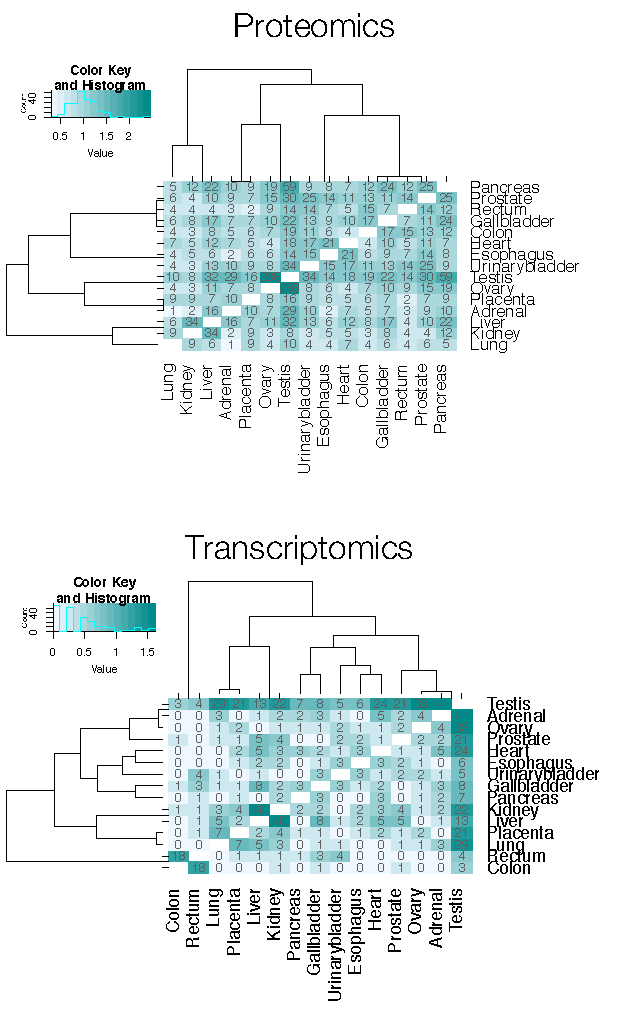
\includegraphics[scale=0.8]{integration/heatmapPairs}\centering
    \caption[Clusters of tissues based on number of proteins or \mRNAs\ shared
    between a pair of tissues]{\label{fig:heatmapPairs}\textbf{Clusters of
    tissues based on number of proteins or \mRNAs\ shared between a pair of
    tissues.} For each pair of tissues, I have collected the number of proteins
    (or \mRNAs) expressed only in that pair. That number is displayed in the
    cell. The heatmap is a symmetric heatmap. Higher is the number of features
    (proteins or \mRNAs) shared between two tissues and closer they are
    considered. We can observe that the tissue presenting the most shared features
    with the other tissues is \tissue{Testis}.}
\end{figure}

\TK{Comparison of the two trees}

\begin{figure}[!htbp]
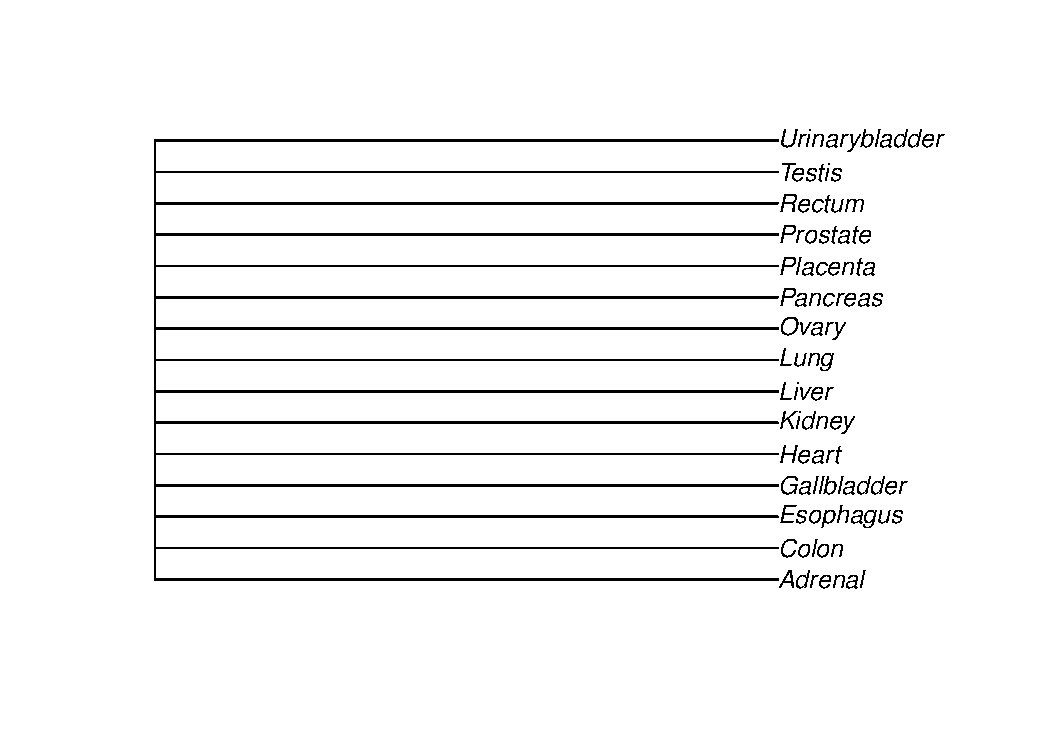
\includegraphics[scale=0.7]{integration/consensusTree}\centering
    \caption[Consensus tree between the cluster trees of the proteome and the
    transcriptome]{\label{fig:consensusTree}\textbf{Consensus tree between the
    cluster trees of the proteome and the transcriptome.}}
\end{figure}

It appears that a direct comparison of the proteins that have been identified
with the identified \mRNAs\ (even with various thresholds) is not so meaningful.

Instead of focusing of the uniqueness of a gene (or in a broader way, the breadth
of expression),the main issue here is to
determine what and when a gene is \emph{specific}. In fact, I can not use
the same definition of detection like for the proteins. I then chose to focus
on the \emph{Tissue-Specific} genes.

\subsection{Tissue specific \textit{m}RNAs have significant overlap with tissue
specific proteins}

\begin{figure}[!htbp]
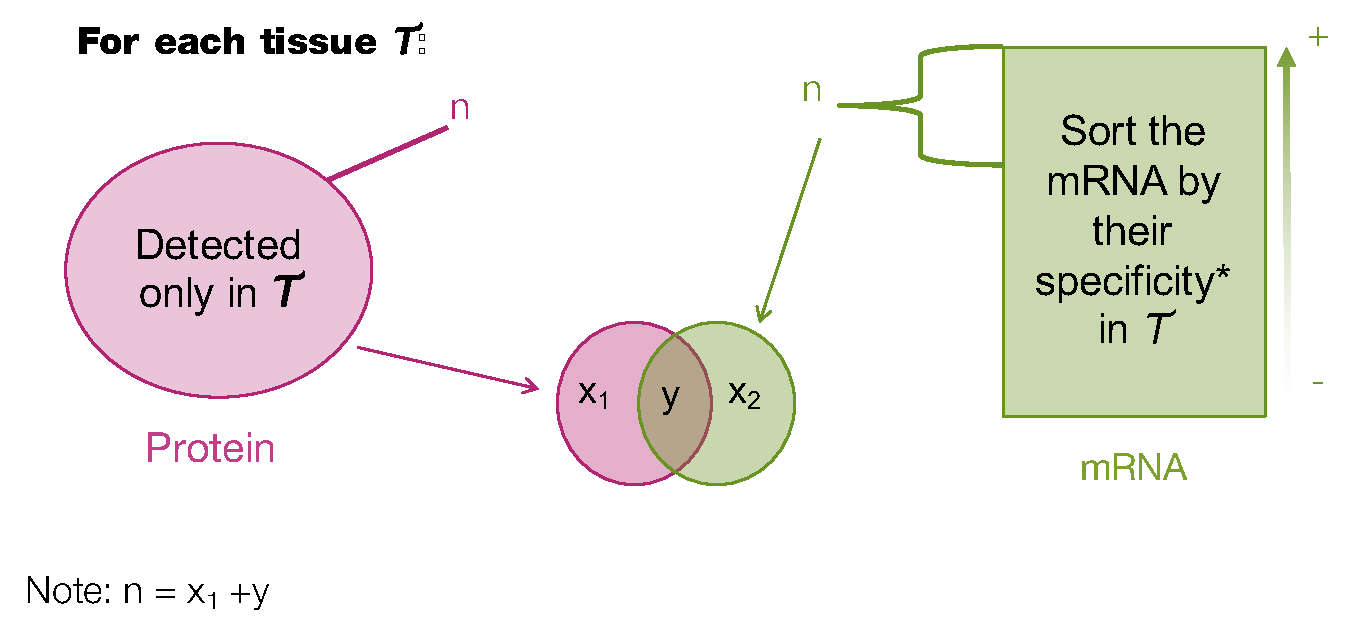
\includegraphics[scale=0.7]{integration/RankSpe}\centering
    \caption[Determination process of specific
    mRNAs]{\label{fig:RankSpe}\textbf{Determination process of specific \mRNAs.}}
\end{figure}


\begin{figure}[!htbp]
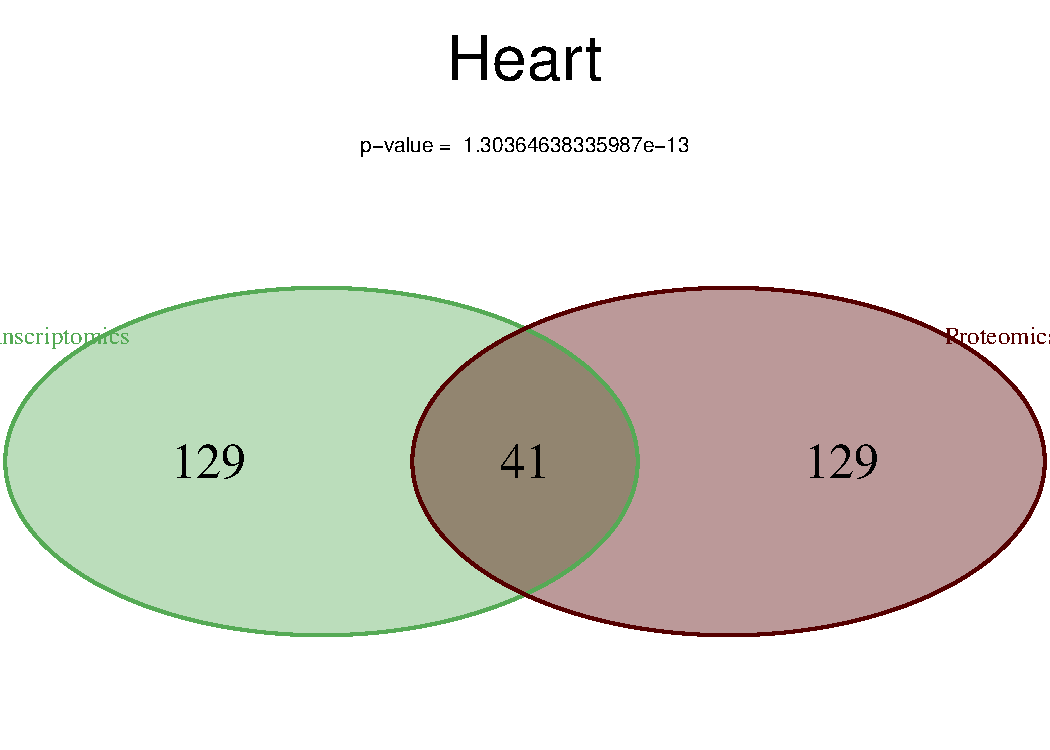
\includegraphics[scale=0.7]{integration/SpeJacquard/Heart}\centering
    \caption[Example of overlap of specific protein and specific
    mRNAs for heart]{\label{fig:ExJacquard}\textbf{Example of overlap of
    specific proteins and specific \mRNAs.}}
\end{figure}


\begin{figure}[!htbp]
\includegraphics[scale=0.4]{integration/RatioJac}\centering
    \caption[Heatmap of Jaquard indices]{\label{fig:RatioJac}\textbf{Heatmap of
    Jaquard indices.}}
\end{figure}

\begin{figure}[!htbp]
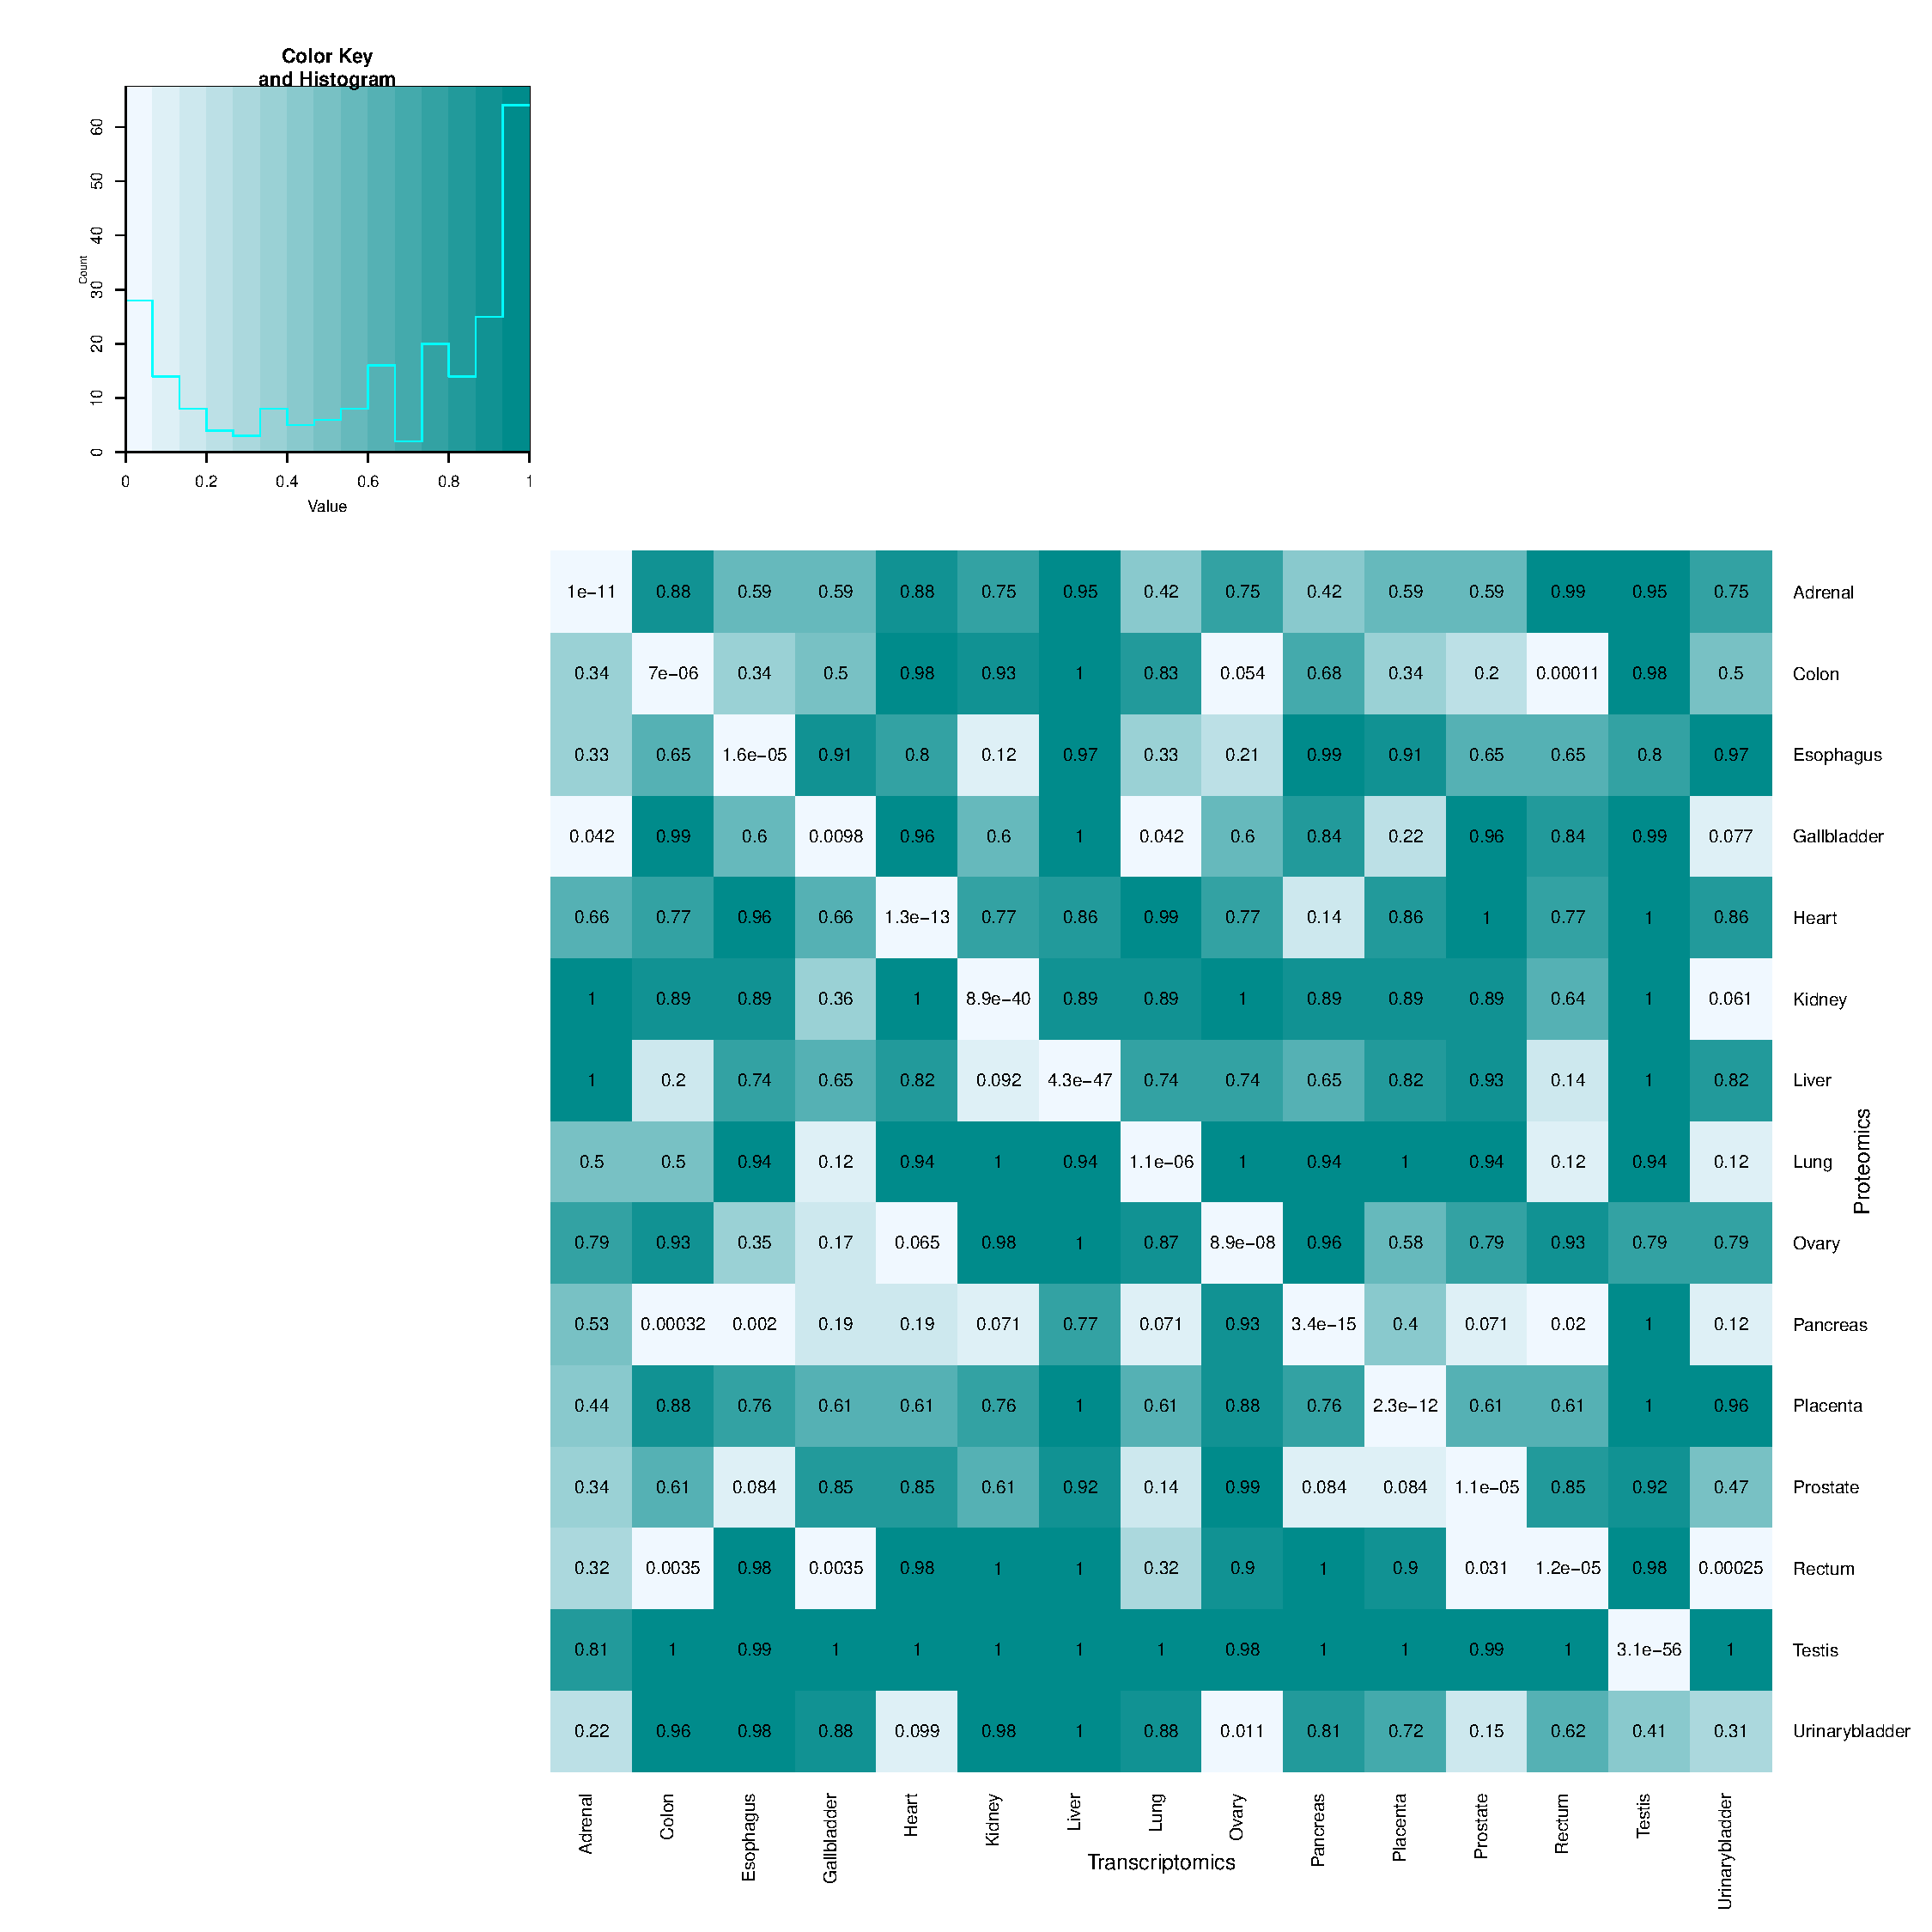
\includegraphics[scale=0.4]{integration/pJacquard}\centering
    \caption[p-values associated to the Jaquard
    indices]{\label{fig:pJacquard}\textbf{p-value associated to the Jaquard
    indices.}They have been computed with hypergeometric test.}
\end{figure}

\subsection{Expression levels of mRNAs correlate with the expressed proteins}

\begin{figure}[!htbp]
    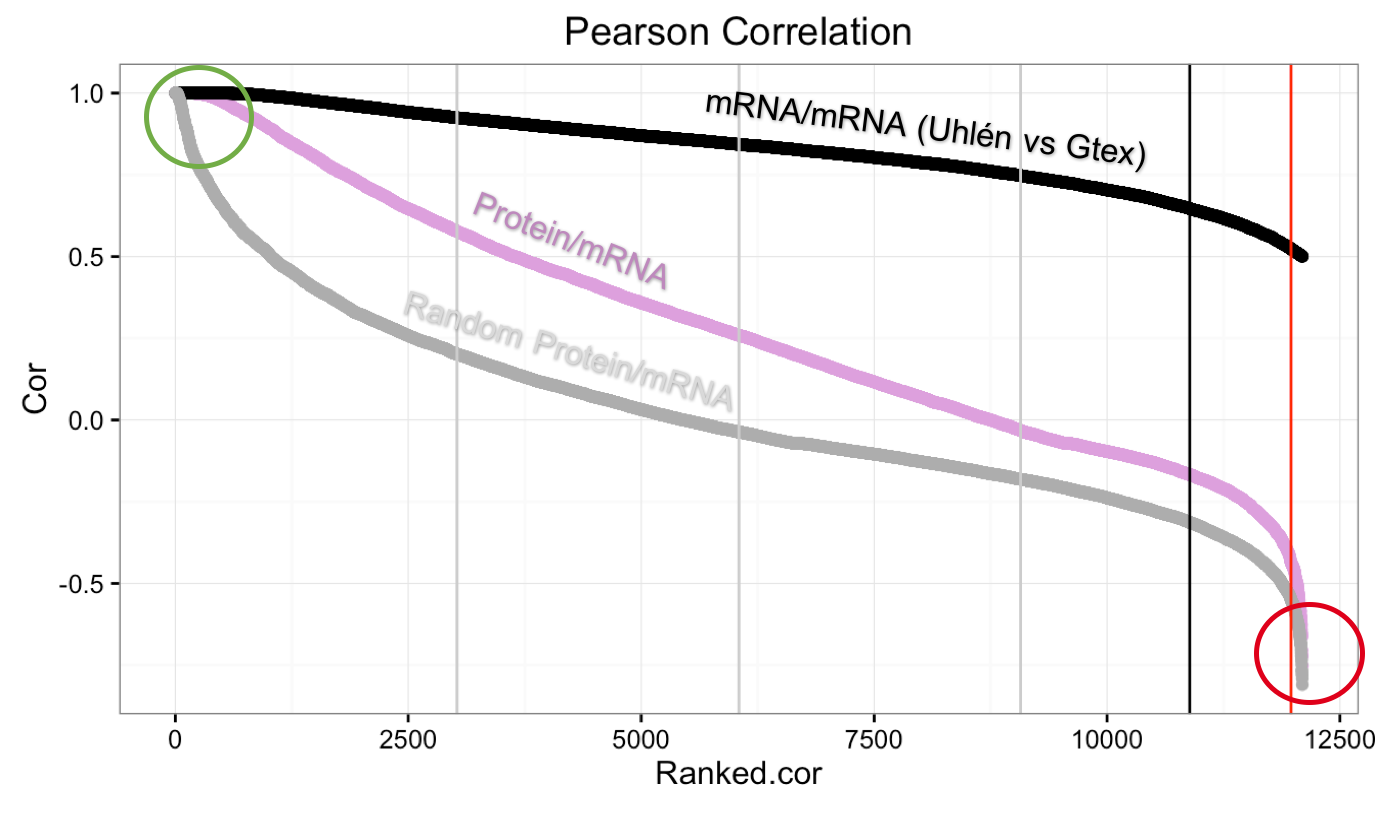
\includegraphics[scale=0.55]{integration/GeneProtCorAnno}\centering
    \caption[Pearson correlation coefficients of \mRNA/protein pairs expression
    across the common tissues in descending order]
    {\label{GeneProtCor}\textbf{Pearson correlation coefficients of \mRNA/protein
    pairs expression across the common tissues in descending order.} For each
    couple of \mRNA\ and its corresponding protein, the Pearson correlation of
    their respective expression across the same set of tissue is calculated. Then,
    all the pairs are sorted in descending order and plotted based on their
    correlation coefficient in pink. To provide context to these results,
    An \emph{ideal} case has also been calculated. The identical \mRNAs\ set of
    the current Proteome and Transcriptome comparison has been used for a
    Transcriptome (\dataset{Uhlén \etal}) and Transcriptome comparison
    (\dataset{GTEX}). We can see that even the ideal case is not a perfect
    horizontal line (which would indicate a whole and complete correlation between
    the two transcriptomic datasets).}
\end{figure}


\begin{figure}[!htbp]
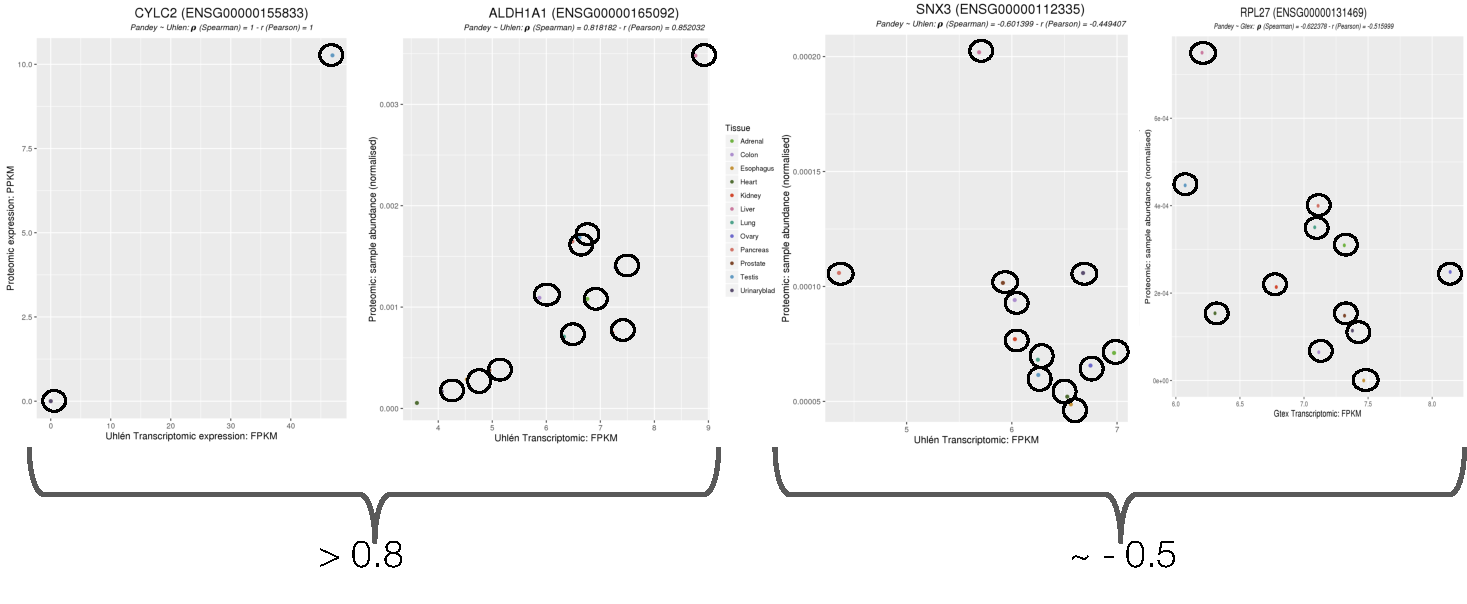
\includegraphics[scale=0.5]{integration/caseGene}\centering
    \caption[Different cases of correlation
    protein/mRNA]{\label{fig:caseGene}\textbf{Different cases of correlation
    protein/\mRNA.} The high correlated ones are enriched in pairs that are
    Tissue-specific as \mRNA\ and protein.}
\end{figure}

\subsection{Pairs composed of tissue specific proteins tend to correlate better}

\begin{figure}[!htbp]
    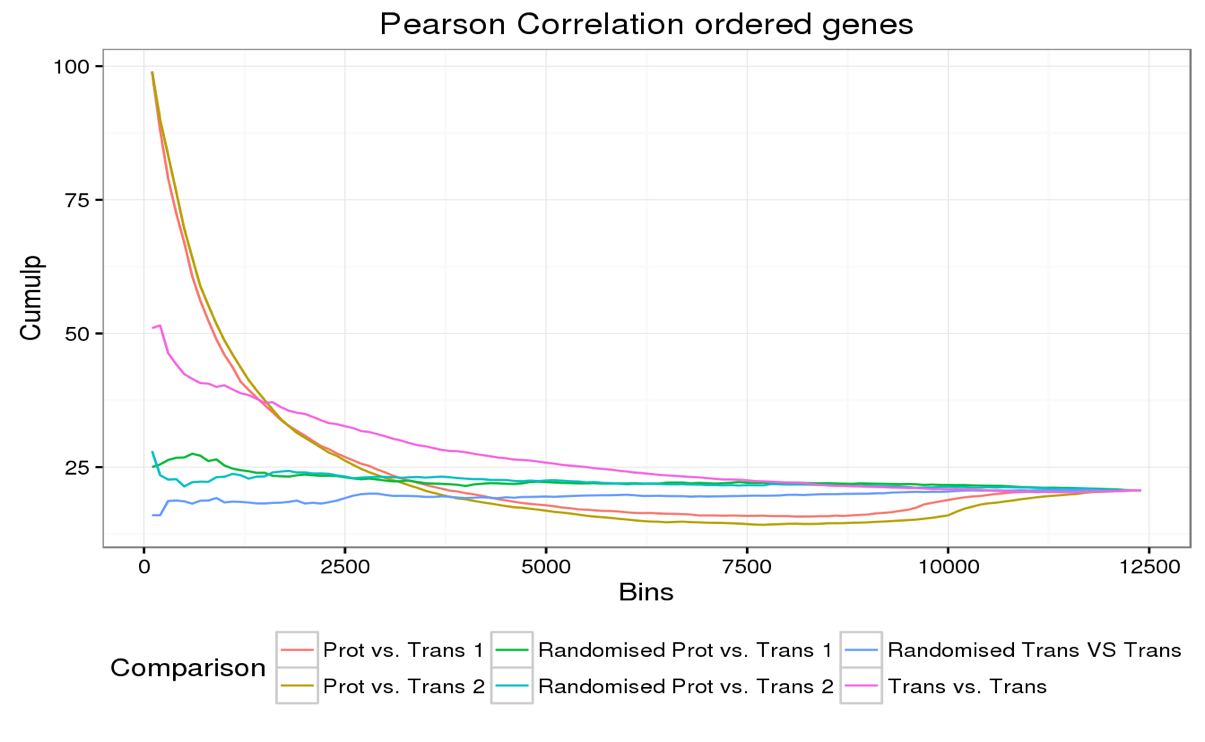
\includegraphics[scale=0.7]{integration/Spe_Cor}\centering
    \caption[Cumul ratio of the specific proteins ordered on the correlation
    of the mRNA/protein pairs across the 15
    tissues]{\label{fig:Spe_Cor}\textbf{Cumul ratio of the specific proteins
    ordered on the correlation of the mRNA/protein pairs across the 15 tissues.}}
\end{figure}


\TK{Can tissues correlations be improved by removing the lowly correlated genes? =>
it is not always the same pairs that are in the same quadrant ==> no `argument''
that would legitimate this. Ref:~\cref{fig:CorImprovable}}


\begin{figure}[!htbp]
    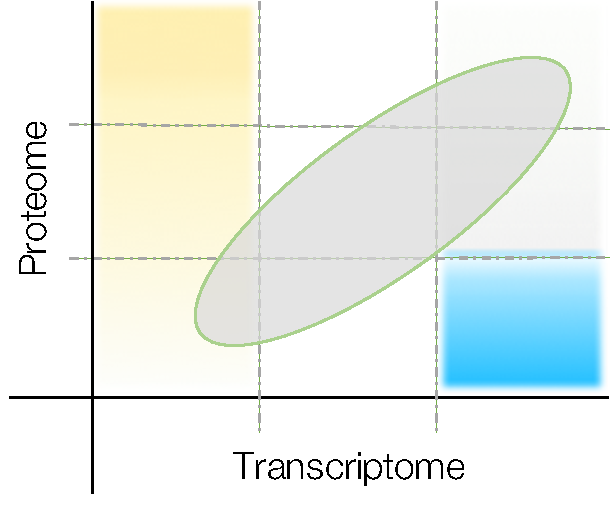
\includegraphics[scale=0.85]{integration/improvingTisseCor}\centering
    \caption[Possible biological significations of a \mRNA/protein pair based on
    its possition in the scatter plot]
    {\label{fig:CorImprovable}\textbf{Possible biological significations of a
    \mRNA/protein pair based on its position in the scatter plot.}Indeed, as all
    the scatter plots present the same shape with a saturation for the proteins
    highly expressed in each tissues and a great dispersion for the lowly
    expressed \mRNAs}
\end{figure}


\subsection{GO enrichment of the different categories}


\begin{figure}[!htbp]
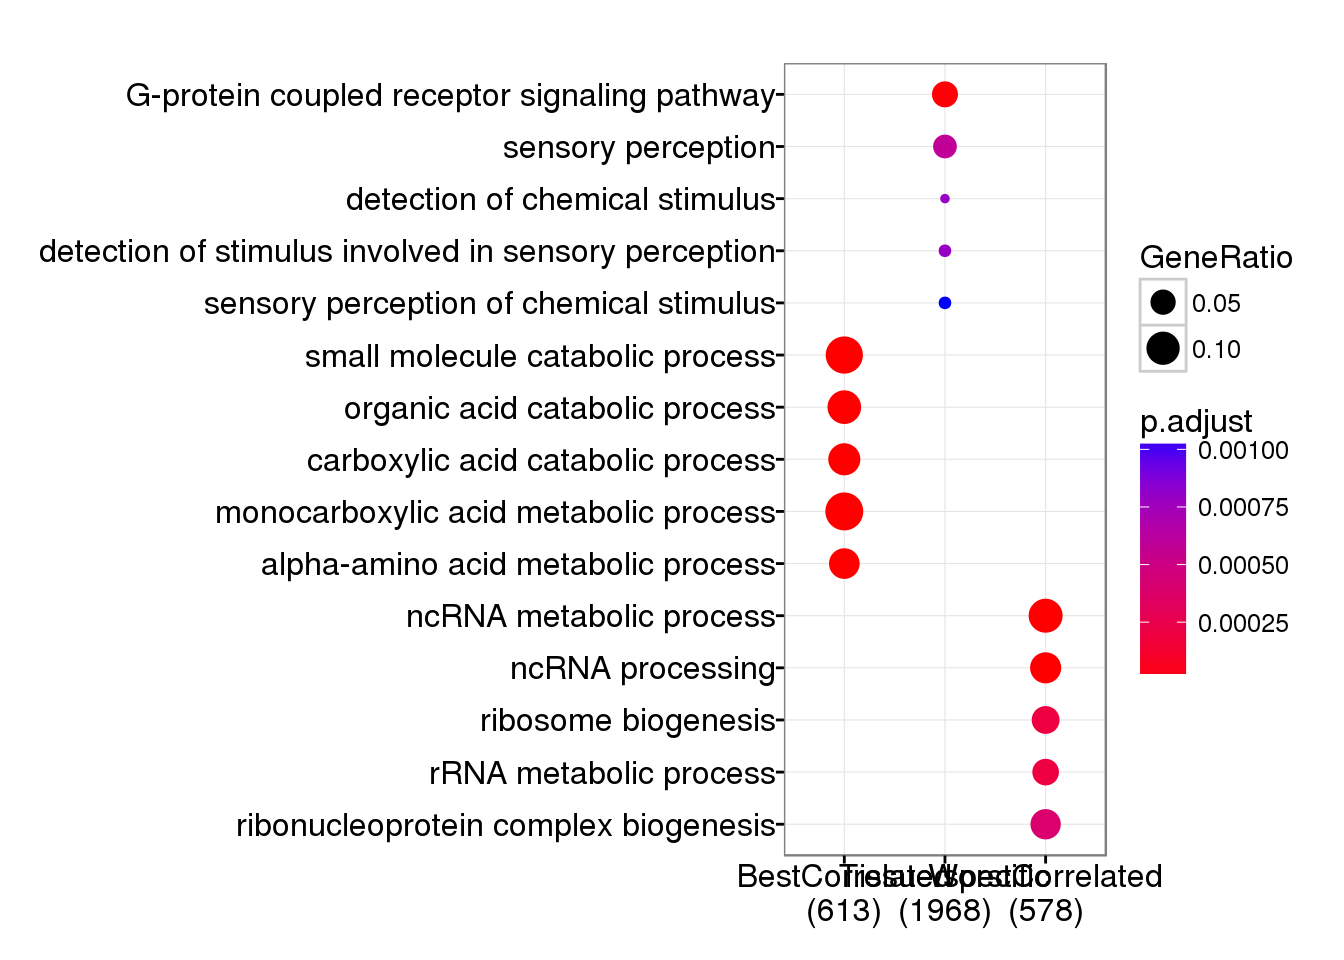
\includegraphics[scale=0.7]{integration/Go_dotplot}\centering
    \caption[GO enrichment analysis of the highest, lowest and Tissue
    specific genes]{\label{fig:Go_dotplot}\textbf{GO enrichment analysis of the
    highest, lowest and Tissue specific genes.}}
\end{figure}


\begin{figure}[!htbp]
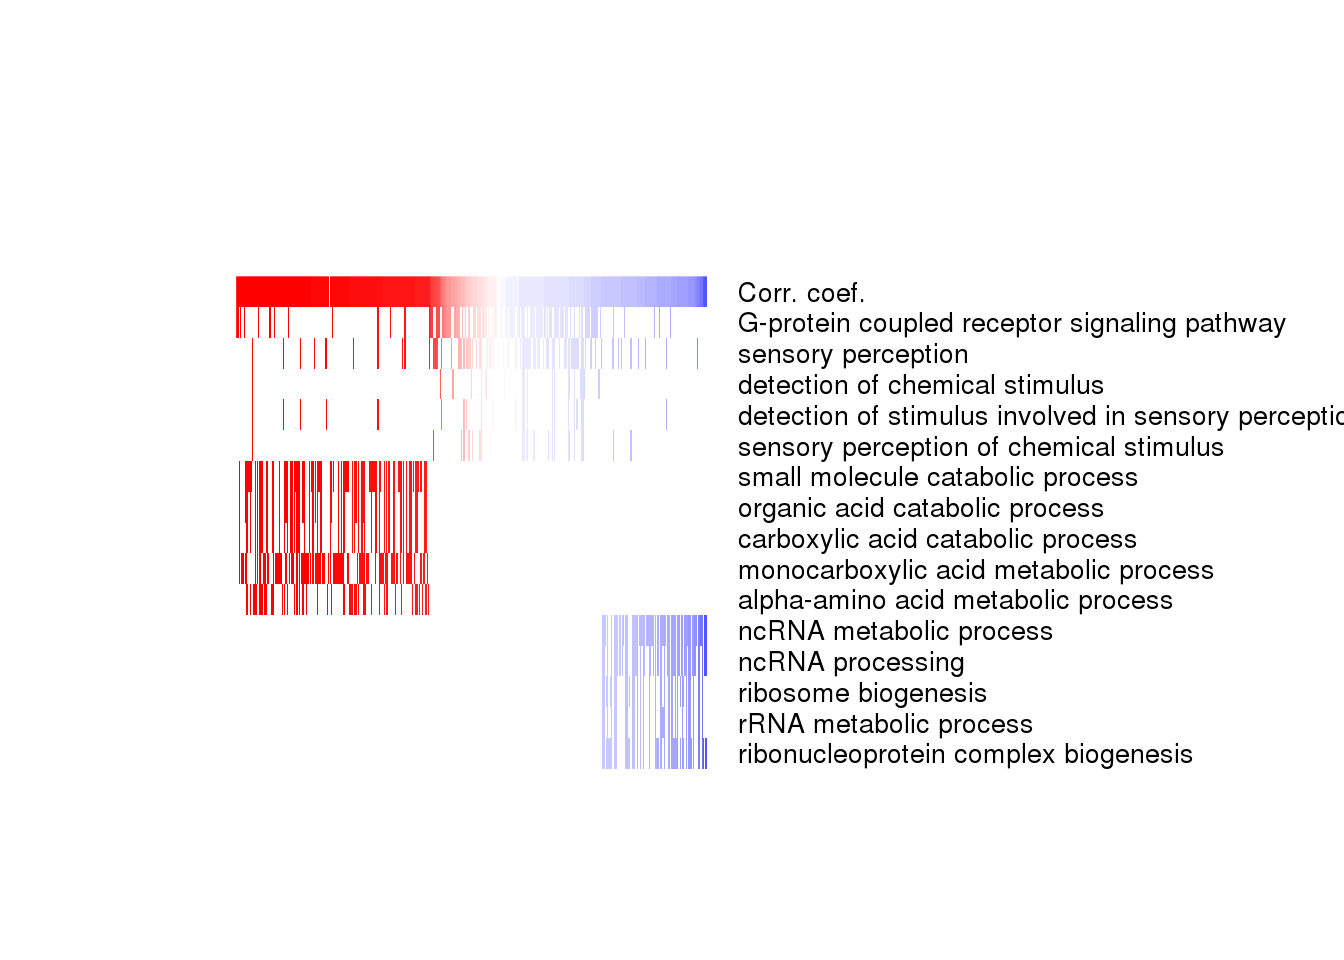
\includegraphics[scale=0.7]{integration/GO_cor_sorted}\centering
    \caption[Correlation coefficient of the pairs for the GO
    categories]{\label{fig:GO_cor_sorted}\textbf{Correlation coefficient of the
    GO categories.}}
\end{figure}


\begin{figure}[!htbp]
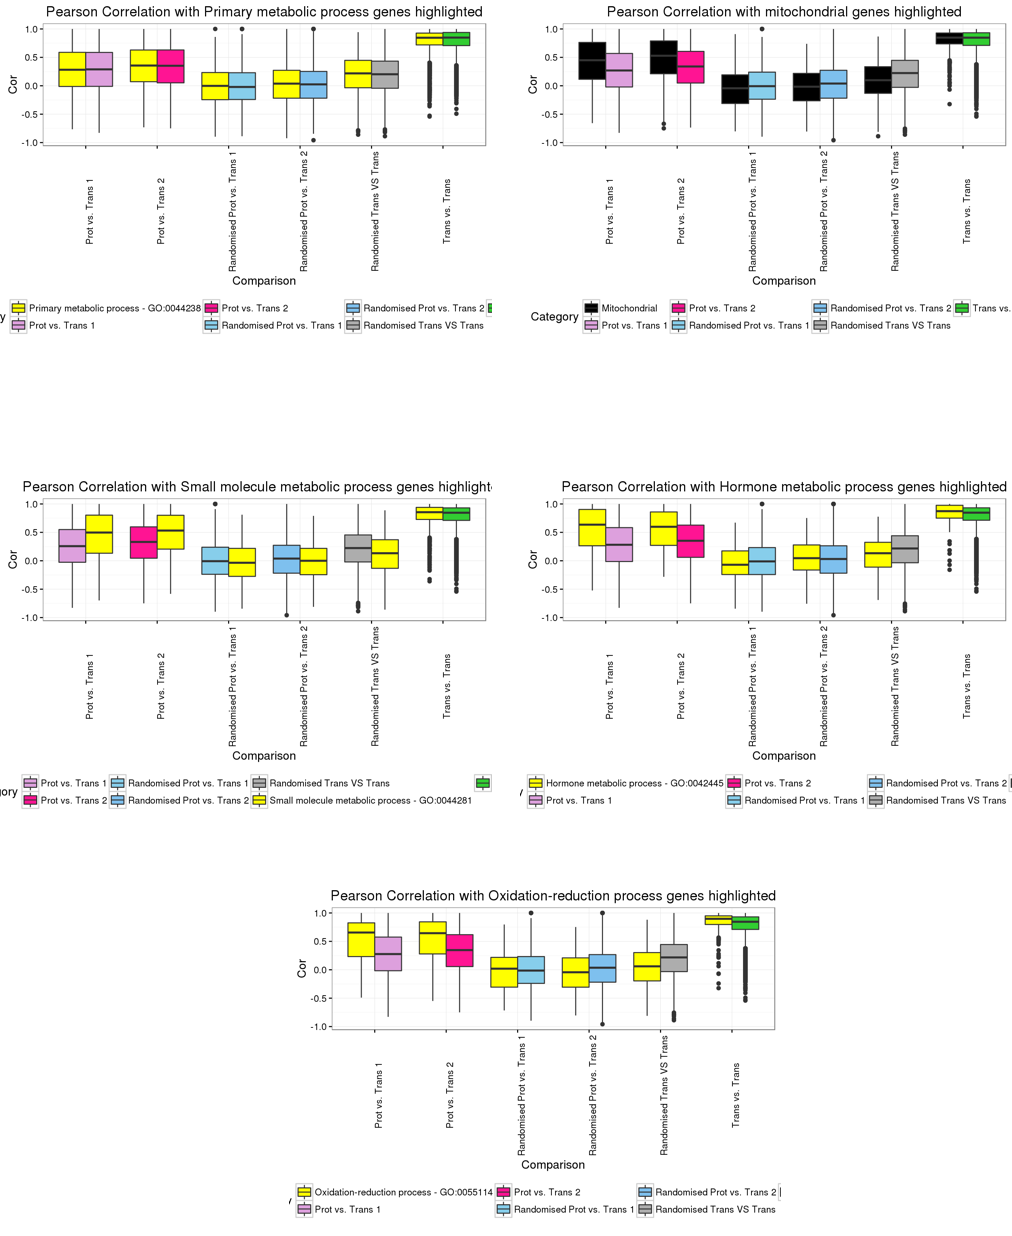
\includegraphics[scale=0.7]{integration/OtherGroups}\centering
    \caption[Examples of particular GO
    categories]{\label{fig:GO_sub_groups}\textbf{Examples of particular GO
    categories.}}
\end{figure}

%\begin{figure}
%    \includegraphics{integration/}\centering
%    \caption[]{\label{} \textbf{}
%    }
%\end{figure}

%if tissue more specific (greater diversity) the proteome, true for transcript as well?
%   barplot (no cutoff) but then 1FPKM<=> 1 protein (barplot 1FPKM ? yes/no?)
%        ---> breadth of expression distribution
%          ---> barplot 5 FPKM ==> Doesn't work BUT other way to compute the
%          specificity of mRNAs--> rank then compute Indice de Jacquard!
%===> *SO* specificity can be kept between Protein and Transcript
%_but then_ quid of Expression values, do they correlate?
%        * Eh, but then show that most high correlated are the specific but not only:
%        there are also others ---> GO annotation.



\clearpage\


\subsection{Annotation + Methodology impact}
\TK{comparison with the Scientific report paper}


\section{Discussion}

Although, the range of Pearson correlation coefficients could seem average or
low, it is actually greater than the average numbers reported in the literature,
\fixme{Add citation list}
particularly as the proteome and the transcriptome have completely different
biological sources.



People look at the highest and lowest expressed genes (in one condition, or very
similar conditions) for the correlation (which is supported by the scatter plot
(indeed, it seems that the greatest bulk is closely correlated) {\Large BUT} if we
want to unlock a deeper understanding of the regulation of the translation, we need
to compare multiple conditions (as all the pairs won't behave in the same fashion
depending which is the considered condition) and more importantly it's it not
really link to the ``quantile'' of expression. Indeed, the protein and the \mRNA\
might be very well correlated, but their expression levels can be somewhat disconnect.

Big plus of this analysis, not only one conditions, but multiple and can try to
avoid technical artefacts by crossing over the results. (More importantly, whatever
which would be found would be consistent with the technology and not just a fling,
i.e.\ it is more robust that any of the study took by itself.)
Which is a weakness of the data (not the same people) create a force (what is found
is probably universal). (We can't say anything about the non-findings!!!)

This ``demarche'' even more important in case that you study the tissue specific
(or condition) specific pair, they globally the more correlated (Are they actually???)

So big need of an external/outliers sample(s) or external source.



%%%%%%%

%%% Check notational for the added Jaquard index analysis and some other stuff.

%%%%%%




%%%%cimetiere
%%These studies however were mostly done at cell levels.
%%While the pool of protein coding transcripts is about 60 to 70 \% similar from
%%one tissue to another, the protein pool is quite different.


% Hence, a component of the decrease in the
% correlation between the \mRNA\ and its protein is due to t The pink line,
%while more similar in essence to the random pair correlation, presents about
%500 genes/proteins pairs that    are highly correlated.


%We can also note that a broader number of tissues-specific \mRNAs\ doesn't
%necessarily imply the same at proteomic level and vice versa.
%In~\cref{fig:barPlotunique}, we can see that \tissue{Testis} and \tissue{Liver}
%are the tissues with the greatest number of tissues specific \mRNAs\ and proteins.
%The reality is more mixed for the other tissues.

%\subsection{Relative specificity of the tissues are kept from transcriptome to
%proteome level for the most extreme cases --- i.e.\ proteomic diversity of a tissue
%can not be systematically deduced from transcriptomic}


%We can also note that a broader number of tissues-specific \mRNAs\ doesn't
%necessarily imply the same at proteomic level and vice versa.
%In~\cref{fig:barPlotunique}, we can see that \tissue{Testis} and \tissue{Liver}
%are the tissues with the greatest number of tissues specific \mRNAs\ and proteins.
%The reality is more mixed for the other tissues.


%As the \mRNAs\ are expressed in more tissues in general, I tried to take account for this in the following analysis I run.
